% Options for packages loaded elsewhere
\PassOptionsToPackage{unicode}{hyperref}
\PassOptionsToPackage{hyphens}{url}
\PassOptionsToPackage{space}{xeCJK}
%
\documentclass[
  9pt,
  ignorenonframetext,
  aspectratio=169,
  t]{beamer}
\usepackage{pgfpages}
\setbeamertemplate{caption}[numbered]
\setbeamertemplate{caption label separator}{: }
\setbeamercolor{caption name}{fg=normal text.fg}
\beamertemplatenavigationsymbolsempty
% Prevent slide breaks in the middle of a paragraph
\widowpenalties 1 10000
\raggedbottom
\setbeamertemplate{part page}{
  \centering
  \begin{beamercolorbox}[sep=16pt,center]{part title}
    \usebeamerfont{part title}\insertpart\par
  \end{beamercolorbox}
}
\setbeamertemplate{section page}{
  \centering
  \begin{beamercolorbox}[sep=12pt,center]{part title}
    \usebeamerfont{section title}\insertsection\par
  \end{beamercolorbox}
}
\setbeamertemplate{subsection page}{
  \centering
  \begin{beamercolorbox}[sep=8pt,center]{part title}
    \usebeamerfont{subsection title}\insertsubsection\par
  \end{beamercolorbox}
}
\AtBeginPart{
  \frame{\partpage}
}
\AtBeginSection{
  \ifbibliography
  \else
    \frame{\sectionpage}
  \fi
}
\AtBeginSubsection{
  \frame{\subsectionpage}
}
\usepackage{amsmath,amssymb}
\usepackage{iftex}
\ifPDFTeX
  \usepackage[T1]{fontenc}
  \usepackage[utf8]{inputenc}
  \usepackage{textcomp} % provide euro and other symbols
\else % if luatex or xetex
  \usepackage{unicode-math} % this also loads fontspec
  \defaultfontfeatures{Scale=MatchLowercase}
  \defaultfontfeatures[\rmfamily]{Ligatures=TeX,Scale=1}
\fi
\usepackage{lmodern}
\usetheme[]{Madrid}
\usefonttheme{serif} % use mainfont rather than sansfont for slide text
\ifPDFTeX\else
  % xetex/luatex font selection
  \setmainfont[]{DejaVu Sans}
  \setmonofont[]{DejaVu Sans Mono}
  \ifXeTeX
    \usepackage{xeCJK}
    \setCJKmainfont[]{Noto Serif CJK SC}
          \fi
  \ifLuaTeX
    \usepackage[]{luatexja-fontspec}
    \setmainjfont[]{Noto Serif CJK SC}
  \fi
\fi
% Use upquote if available, for straight quotes in verbatim environments
\IfFileExists{upquote.sty}{\usepackage{upquote}}{}
\IfFileExists{microtype.sty}{% use microtype if available
  \usepackage[]{microtype}
  \UseMicrotypeSet[protrusion]{basicmath} % disable protrusion for tt fonts
}{}
\makeatletter
\@ifundefined{KOMAClassName}{% if non-KOMA class
  \IfFileExists{parskip.sty}{%
    \usepackage{parskip}
  }{% else
    \setlength{\parindent}{0pt}
    \setlength{\parskip}{6pt plus 2pt minus 1pt}}
}{% if KOMA class
  \KOMAoptions{parskip=half}}
\makeatother
\usepackage{xcolor}
\newif\ifbibliography
\usepackage{color}
\usepackage{fancyvrb}
\newcommand{\VerbBar}{|}
\newcommand{\VERB}{\Verb[commandchars=\\\{\}]}
\DefineVerbatimEnvironment{Highlighting}{Verbatim}{commandchars=\\\{\}}
% Add ',fontsize=\small' for more characters per line
\newenvironment{Shaded}{}{}
\newcommand{\AlertTok}[1]{\textcolor[rgb]{1.00,0.00,0.00}{\textbf{#1}}}
\newcommand{\AnnotationTok}[1]{\textcolor[rgb]{0.38,0.63,0.69}{\textbf{\textit{#1}}}}
\newcommand{\AttributeTok}[1]{\textcolor[rgb]{0.49,0.56,0.16}{#1}}
\newcommand{\BaseNTok}[1]{\textcolor[rgb]{0.25,0.63,0.44}{#1}}
\newcommand{\BuiltInTok}[1]{\textcolor[rgb]{0.00,0.50,0.00}{#1}}
\newcommand{\CharTok}[1]{\textcolor[rgb]{0.25,0.44,0.63}{#1}}
\newcommand{\CommentTok}[1]{\textcolor[rgb]{0.38,0.63,0.69}{\textit{#1}}}
\newcommand{\CommentVarTok}[1]{\textcolor[rgb]{0.38,0.63,0.69}{\textbf{\textit{#1}}}}
\newcommand{\ConstantTok}[1]{\textcolor[rgb]{0.53,0.00,0.00}{#1}}
\newcommand{\ControlFlowTok}[1]{\textcolor[rgb]{0.00,0.44,0.13}{\textbf{#1}}}
\newcommand{\DataTypeTok}[1]{\textcolor[rgb]{0.56,0.13,0.00}{#1}}
\newcommand{\DecValTok}[1]{\textcolor[rgb]{0.25,0.63,0.44}{#1}}
\newcommand{\DocumentationTok}[1]{\textcolor[rgb]{0.73,0.13,0.13}{\textit{#1}}}
\newcommand{\ErrorTok}[1]{\textcolor[rgb]{1.00,0.00,0.00}{\textbf{#1}}}
\newcommand{\ExtensionTok}[1]{#1}
\newcommand{\FloatTok}[1]{\textcolor[rgb]{0.25,0.63,0.44}{#1}}
\newcommand{\FunctionTok}[1]{\textcolor[rgb]{0.02,0.16,0.49}{#1}}
\newcommand{\ImportTok}[1]{\textcolor[rgb]{0.00,0.50,0.00}{\textbf{#1}}}
\newcommand{\InformationTok}[1]{\textcolor[rgb]{0.38,0.63,0.69}{\textbf{\textit{#1}}}}
\newcommand{\KeywordTok}[1]{\textcolor[rgb]{0.00,0.44,0.13}{\textbf{#1}}}
\newcommand{\NormalTok}[1]{#1}
\newcommand{\OperatorTok}[1]{\textcolor[rgb]{0.40,0.40,0.40}{#1}}
\newcommand{\OtherTok}[1]{\textcolor[rgb]{0.00,0.44,0.13}{#1}}
\newcommand{\PreprocessorTok}[1]{\textcolor[rgb]{0.74,0.48,0.00}{#1}}
\newcommand{\RegionMarkerTok}[1]{#1}
\newcommand{\SpecialCharTok}[1]{\textcolor[rgb]{0.25,0.44,0.63}{#1}}
\newcommand{\SpecialStringTok}[1]{\textcolor[rgb]{0.73,0.40,0.53}{#1}}
\newcommand{\StringTok}[1]{\textcolor[rgb]{0.25,0.44,0.63}{#1}}
\newcommand{\VariableTok}[1]{\textcolor[rgb]{0.10,0.09,0.49}{#1}}
\newcommand{\VerbatimStringTok}[1]{\textcolor[rgb]{0.25,0.44,0.63}{#1}}
\newcommand{\WarningTok}[1]{\textcolor[rgb]{0.38,0.63,0.69}{\textbf{\textit{#1}}}}
\usepackage{longtable,booktabs,array}
\usepackage{calc} % for calculating minipage widths
\usepackage{caption}
% Make caption package work with longtable
\makeatletter
\def\fnum@table{\tablename~\thetable}
\makeatother
\setlength{\emergencystretch}{3em} % prevent overfull lines
\providecommand{\tightlist}{%
  \setlength{\itemsep}{0pt}\setlength{\parskip}{0pt}}
\setcounter{secnumdepth}{-\maxdimen} % remove section numbering
% Tighten vertical rhythm so dense slides fit on a single frame.
\usepackage{etoolbox}
% TikZ so the ported reference diagrams render (same libraries as the report).
\usepackage{tikz}
\usetikzlibrary{arrows.meta,positioning,fit,backgrounds}
% A standalone section title slide at the start of each section (# headers),
% plus the \tableofcontents on the Outline slide, give the deck its structure.
\AtBeginSection[]{\frame{\sectionpage}}
\setbeamertemplate{section in toc}[sections numbered]
\setlength{\parskip}{3pt plus 1pt minus 1pt}
\setbeamertemplate{itemize/enumerate body begin}{\small}
\setbeamertemplate{itemize/enumerate subbody begin}{\footnotesize}
\AtBeginEnvironment{itemize}{\setlength{\itemsep}{2pt}\setlength{\topsep}{2pt}}
\AtBeginEnvironment{enumerate}{\setlength{\itemsep}{2pt}\setlength{\topsep}{2pt}}
\AtBeginEnvironment{Highlighting}{\footnotesize}
\AtBeginEnvironment{verbatim}{\footnotesize}
\AtBeginEnvironment{longtable}{\scriptsize}
% longtable's default pre/post glue is \bigskip; trim it so the trailing
% "-> Report" pointer stays on the table's own frame instead of spilling.
\setlength\LTpre{2pt}\setlength\LTpost{2pt}
\ifLuaTeX
  \usepackage{selnolig}  % disable illegal ligatures
\fi
\IfFileExists{bookmark.sty}{\usepackage{bookmark}}{\usepackage{hyperref}}
\IfFileExists{xurl.sty}{\usepackage{xurl}}{} % add URL line breaks if available
\urlstyle{same}
\hypersetup{
  pdftitle={AgentCore as the Sandbox in Agentic RL},
  pdfauthor={Kaige Yang --- Senior Applied Scientist, AWS},
  hidelinks,
  pdfcreator={LaTeX via pandoc}}

\title{AgentCore as the Sandbox in Agentic RL}
\subtitle{AgentCore Runtime as the execution sandbox, integrated with
slime}
\author{Kaige Yang --- Senior Applied Scientist, AWS}
\date{September 10, 2026}

\setbeamertemplate{frametitle continuation}[from second]
\begin{document}
\frame{\titlepage}

\begin{frame}[allowframebreaks]{Outline}
\protect\hypertarget{outline}{}
\tableofcontents
\end{frame}

\hypertarget{why-sandboxes-what-frontier-labs-run-in-them}{%
\section{1. Why sandboxes --- what frontier labs run in
them}\label{why-sandboxes-what-frontier-labs-run-in-them}}

\begin{frame}[allowframebreaks]{Purpose \& roadmap --- AgentCore as the sandbox for
agentic RL}
\protect\hypertarget{purpose-roadmap-agentcore-as-the-sandbox-for-agentic-rl}{}
\textbf{One idea:} in agentic RL the policy acts over many turns against
an executable environment, and a \textbf{programmatic checker} --- not
an LLM judge --- turns the outcome into a scalar reward (RLVR).

\textbf{Roadmap (6 sections):}

\begin{enumerate}
\tightlist
\item
  \textbf{Why sandboxes} --- what frontier labs run in sandboxes, and
  how they score it.
\item
  \textbf{Architecture \& pipeline} --- reference architecture, the five
  components, TITO, slime + its async rollout.
\item
  \textbf{Foundations of AgentCore} --- Runtime / session / microVM, CPU
  vs GPU compute, session lifecycle \& launch/terminate.
\item
  \textbf{Integrating into slime} --- the call path, one hook, the
  episode loop, and the key code.
\item
  \textbf{The demos} --- all 21 at a glance, each with its real use
  case.
\item
  \textbf{Special demos} --- scaling (harness × inference × sandbox),
  mixed-task, GPU sharing, image pool, real-CLI branching, heartbeat.
\end{enumerate}

\emph{Scope: AgentCore = the execution \textbf{sandbox}; \textbf{slime}
= the trainer; the \textbf{harness stays in-process}.}
\end{frame}

\begin{frame}[allowframebreaks]{What tasks do frontier labs run in sandboxes}
\protect\hypertarget{what-tasks-do-frontier-labs-run-in-sandboxes}{}
Untrusted output runs in an isolated sandbox; a \textbf{programmatic
verifier} produces the reward. This is the dominant recipe in recent
tech reports --- Kimi K2 {[}5{]} reports \textbf{\textgreater10,000
concurrent sandboxes} for agentic tool-use / code RL.

\textbf{Two verifier styles:} \emph{verifiable / rule-based} (binary,
ungameable) vs \emph{reference-based judge} (open-ended). This project
uses \textbf{RLVR only}.

\begin{longtable}[]{@{}
  >{\raggedright\arraybackslash}p{(\columnwidth - 6\tabcolsep) * \real{0.2500}}
  >{\raggedright\arraybackslash}p{(\columnwidth - 6\tabcolsep) * \real{0.2500}}
  >{\raggedright\arraybackslash}p{(\columnwidth - 6\tabcolsep) * \real{0.2500}}
  >{\raggedright\arraybackslash}p{(\columnwidth - 6\tabcolsep) * \real{0.2500}}@{}}
\toprule\noalign{}
\begin{minipage}[b]{\linewidth}\raggedright
Model
\end{minipage} & \begin{minipage}[b]{\linewidth}\raggedright
Verifier
\end{minipage} & \begin{minipage}[b]{\linewidth}\raggedright
Tasks
\end{minipage} & \begin{minipage}[b]{\linewidth}\raggedright
Reward
\end{minipage} \\
\midrule\noalign{}
\endhead
DeepSeek-R1 {[}2{]} & rule verifier + compiler & math, competitive code
& tests pass / match \\
Qwen3 {[}3{]} & RLVR + live tool env & math, code, tool-use, RAG & rule
+ judge \\
Llama-Nemotron {[}4{]} & LLM-judge & science, math, instruction & match
+ format \\
Kimi K2 {[}5{]} & simulator + real exec sandboxes & agentic tool use,
code, SWE & tests + checks \\
\bottomrule\noalign{}
\end{longtable}

\emph{Same recipe throughout this deck: \textbf{one isolated sandbox per
episode}, a \textbf{programmatic checker} for the reward.}
\end{frame}

\hypertarget{agentic-rl-architecture-the-training-pipeline}{%
\section{2. Agentic RL architecture \& the training
pipeline}\label{agentic-rl-architecture-the-training-pipeline}}

\begin{frame}[allowframebreaks]{The reference architecture --- one diagram}
\protect\hypertarget{the-reference-architecture-one-diagram}{}
\begin{center}
\resizebox{\textwidth}{!}{%
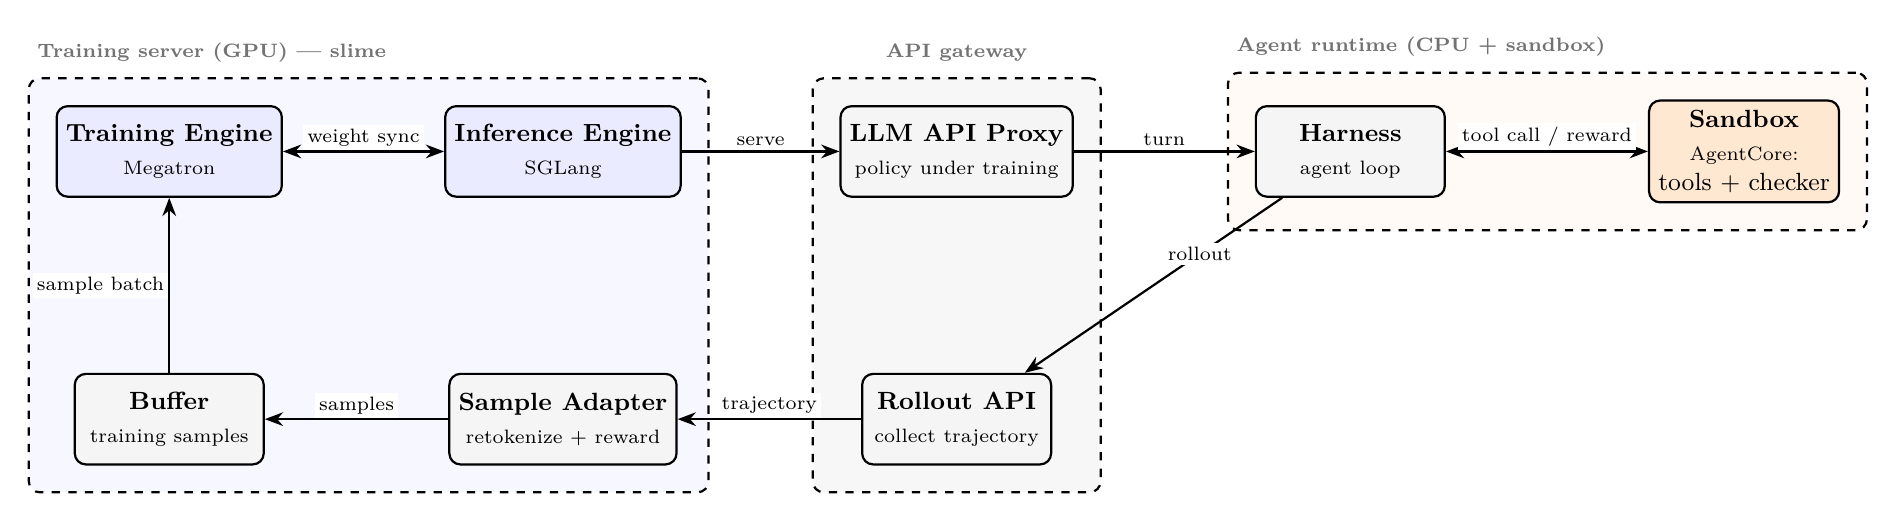
\begin{tikzpicture}[
  font=\small,
  box/.style={draw, rounded corners, minimum height=1.15cm, minimum width=2.4cm, align=center, thick, fill=white},
  gpu/.style={box, fill=blue!8},
  cpu/.style={box, fill=black!4},
  focus/.style={box, fill=orange!18},
  lbl/.style={font=\scriptsize, align=center, fill=white, inner sep=1.5pt},
  ptitle/.style={font=\scriptsize\bfseries, text=black!55},
  panel/.style={draw, rounded corners, dashed, thick, inner sep=0.34cm},
  >={Stealth[]},
]
\node[gpu] (trainer) at (0,0)    {\textbf{Training Engine}\\[1pt]\scriptsize Megatron};
\node[gpu] (infer)   at (5.0,0)  {\textbf{Inference Engine}\\[1pt]\scriptsize SGLang};
\node[cpu] (buffer)  at (0,-3.4) {\textbf{Buffer}\\[1pt]\scriptsize training samples};
\node[cpu] (adapter) at (5.0,-3.4){\textbf{Sample Adapter}\\[1pt]\scriptsize retokenize + reward};
\node[cpu] (proxy)   at (10.0,0)   {\textbf{LLM API Proxy}\\[1pt]\scriptsize policy under training};
\node[cpu] (rollout) at (10.0,-3.4){\textbf{Rollout API}\\[1pt]\scriptsize collect trajectory};
\node[cpu]   (harness) at (15.0,0) {\textbf{Harness}\\[1pt]\scriptsize agent loop};
\node[focus] (sandbox) at (20.0,0){\textbf{Sandbox}\\[1pt]\scriptsize AgentCore:\\tools + checker};
\draw[<->, thick] (trainer) -- node[lbl,above]{weight sync} (infer);
\draw[->, thick]  (infer)   -- node[lbl,above]{serve} (proxy);
\draw[->, thick]  (proxy)   -- node[lbl,above]{turn} (harness);
\draw[<->, thick] (harness) -- node[lbl,above]{tool call / reward} (sandbox);
\draw[->, thick]  (harness) -- node[lbl,pos=0.32]{rollout} (rollout);
\draw[->, thick]  (rollout) -- node[lbl,above]{trajectory} (adapter);
\draw[->, thick]  (adapter) -- node[lbl,above]{samples} (buffer);
\draw[->, thick]  (buffer)  -- node[lbl,left]{sample batch} (trainer);
\begin{scope}[on background layer]
  \node[panel, fill=blue!3,  fit=(trainer)(infer)(buffer)(adapter)] (ptrain) {};
  \node[panel, fill=black!3, fit=(proxy)(rollout)] (pgw) {};
  \node[panel, fill=orange!4, fit=(harness)(sandbox)] (pagent) {};
\end{scope}
\node[ptitle, anchor=south west] at ([yshift=2pt]ptrain.north west) {Training server (GPU) --- slime};
\node[ptitle, anchor=south] at ([yshift=2pt]pgw.north) {API gateway};
\node[ptitle, anchor=south west] at ([yshift=2pt]pagent.north west) {Agent runtime (CPU + sandbox)};
\end{tikzpicture}%
}
\end{center}

\emph{Generation lane (top, →); training-data lane (bottom, ←);
disaggregated design after Agent Lightning {[}1{]}, slime {[}9{]} as
trainer. \textbf{AgentCore fills the sandbox seam.}}
\end{frame}

\begin{frame}[allowframebreaks]{The pipeline --- five components, one job each}
\protect\hypertarget{the-pipeline-five-components-one-job-each}{}
\begin{itemize}
\tightlist
\item
  \textbf{Trainer / Inference} (GPU) --- learn, and generate turns at
  the \emph{current} policy (kept fresh by \textbf{weight sync}).
\item
  \textbf{Proxy} (CPU) --- makes every model call hit the \emph{policy
  under training}, not an external API.
\item
  \textbf{Harness} (CPU) --- the agent loop that owns one episode
  end-to-end.
\item
  \textbf{Sandbox} (CPU/GPU) --- the isolated box untrusted output runs
  in; the \textbf{checker scores the reward}.
\end{itemize}

\textbf{Two lanes, one cycle:}

\begin{itemize}
\tightlist
\item
  \textbf{Generation lane (→):} trainer weights → SGLang → proxy →
  harness turn → sandbox tool call → observation → next turn.
\item
  \textbf{Training-data lane (←):} trajectory → reward attached →
  loss-masked sample → buffer → trainer step → weight sync.
\end{itemize}

\textbf{AgentCore fills the sandbox seam} --- ad-hoc + isolated per
episode. The harness needs \emph{warmth}, not isolation, so it stays
\textbf{in-process}.
\end{frame}

\begin{frame}[fragile,allowframebreaks]{TITO --- why the proxy exists}
\protect\hypertarget{tito-why-the-proxy-exists}{}
A harness works in \textbf{text}; RL trains on \textbf{token IDs}.
Re-tokenizing decoded text can drift from what the model actually
sampled --- corrupting the action, the importance ratio, and the loss
mask.

\begin{center}
\resizebox{0.82\textwidth}{!}{%
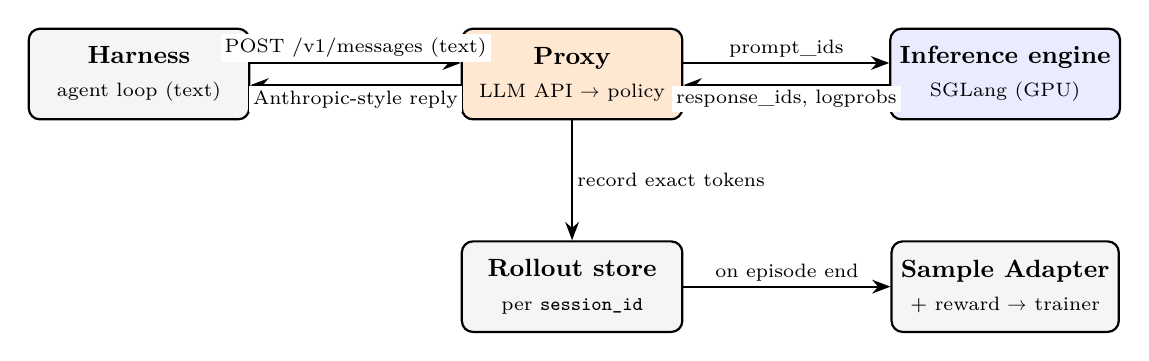
\begin{tikzpicture}[
  font=\small,
  box/.style={draw, rounded corners, minimum height=1.15cm, minimum width=2.8cm, align=center, thick, fill=white},
  svc/.style={box, fill=blue!8},
  focus/.style={box, fill=orange!18},
  cpu/.style={box, fill=black!4},
  lbl/.style={font=\scriptsize, align=center, fill=white, inner sep=1.5pt},
  >={Stealth[]},
]
\node[cpu]   (harness) at (0,0)     {\textbf{Harness}\\[1pt]\scriptsize agent loop (text)};
\node[focus] (proxy)   at (5.5,0)   {\textbf{Proxy}\\[1pt]\scriptsize LLM API $\rightarrow$ policy};
\node[svc]   (infer)   at (11.0,0)  {\textbf{Inference engine}\\[1pt]\scriptsize SGLang (GPU)};
\node[cpu]   (store)   at (5.5,-2.7) {\textbf{Rollout store}\\[1pt]\scriptsize per \texttt{session\_id}};
\node[cpu]   (adapter) at (11.0,-2.7){\textbf{Sample Adapter}\\[1pt]\scriptsize + reward $\rightarrow$ trainer};
\draw[->, thick] ([yshift=4pt]harness.east) -- node[lbl,above]{POST /v1/messages (text)} ([yshift=4pt]proxy.west);
\draw[->, thick] ([yshift=-4pt]proxy.west)  -- node[lbl,below]{Anthropic-style reply} ([yshift=-4pt]harness.east);
\draw[->, thick] ([yshift=4pt]proxy.east) -- node[lbl,above]{prompt\_ids} ([yshift=4pt]infer.west);
\draw[->, thick] ([yshift=-4pt]infer.west) -- node[lbl,below]{response\_ids, logprobs} ([yshift=-4pt]proxy.east);
\draw[->, thick] (proxy) -- node[lbl,right]{record exact tokens} (store);
\draw[->, thick] (store) -- node[lbl,above]{on episode end} (adapter);
\end{tikzpicture}%
}
\end{center}

\textbf{Token-in-token-out (TITO):} the proxy records the \textbf{exact
sampled \texttt{token\_ids} + logprobs} at generation time and forwards
them intact, so the trainer learns from the tokens that were really
sampled.

\begin{itemize}
\tightlist
\item
  The proxy is the only component straddling both sides (text ↔ tokens),
  so it is the only correct place to capture them.
\item
  For binary RLVR rewards this token-level exactness is not optional ---
  slop silently corrupts the signal.
\end{itemize}
\end{frame}

\begin{frame}[fragile,allowframebreaks]{slime --- the trainer, and its asynchronous
rollout}
\protect\hypertarget{slime-the-trainer-and-its-asynchronous-rollout}{}
\begin{center}
\resizebox{0.5\textwidth}{!}{%
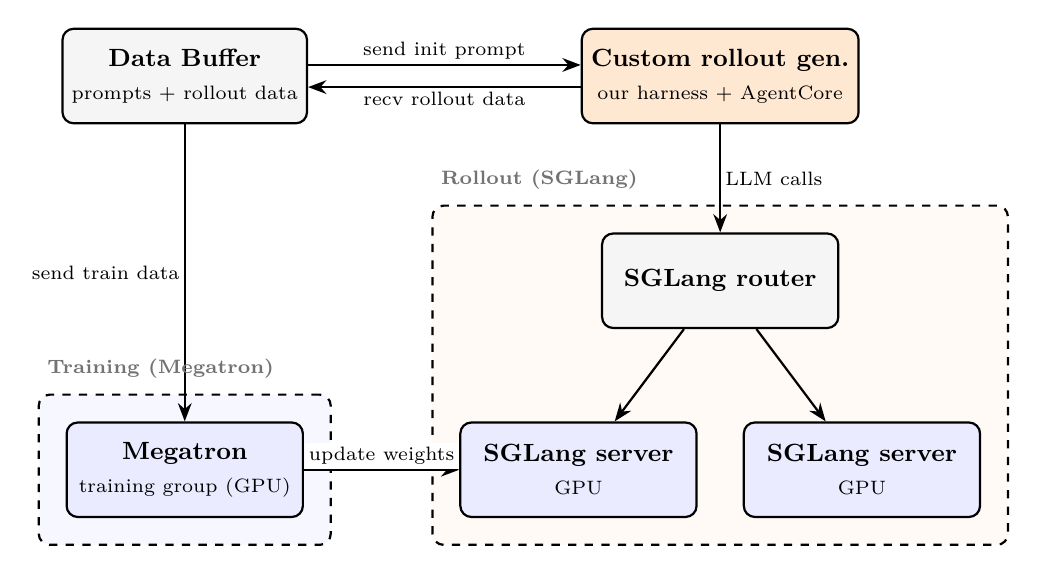
\begin{tikzpicture}[
  font=\small,
  box/.style={draw, rounded corners, minimum height=1.2cm, minimum width=3.0cm, align=center, thick, fill=white},
  gpu/.style={box, fill=blue!8},
  cpu/.style={box, fill=black!4},
  focus/.style={box, fill=orange!18},
  lbl/.style={font=\scriptsize, align=center, fill=white, inner sep=1.5pt},
  ptitle/.style={font=\scriptsize\bfseries, text=black!55},
  panel/.style={draw, rounded corners, dashed, thick, inner sep=0.34cm},
  >={Stealth[]},
]
\node[cpu]   (buffer)  at (0,0)      {\textbf{Data Buffer}\\[1pt]\scriptsize prompts + rollout data};
\node[focus] (rollout) at (6.8,0)    {\textbf{Custom rollout gen.}\\[1pt]\scriptsize our harness + AgentCore};
\node[cpu]   (router)  at (6.8,-2.6) {\textbf{SGLang router}};
\node[gpu]   (sg1)     at (5.0,-5.0) {\textbf{SGLang server}\\[1pt]\scriptsize GPU};
\node[gpu]   (sg2)     at (8.6,-5.0) {\textbf{SGLang server}\\[1pt]\scriptsize GPU};
\node[gpu]   (mega)    at (0,-5.0)   {\textbf{Megatron}\\[1pt]\scriptsize training group (GPU)};
\draw[->, thick] ([yshift=4pt]buffer.east) -- node[lbl,above]{send init prompt} ([yshift=4pt]rollout.west);
\draw[->, thick] ([yshift=-4pt]rollout.west) -- node[lbl,below]{recv rollout data} ([yshift=-4pt]buffer.east);
\draw[->, thick] (rollout) -- node[lbl,right]{LLM calls} (router);
\draw[->, thick] (router)  -- (sg1);
\draw[->, thick] (router)  -- (sg2);
\draw[->, thick] (buffer)  -- node[lbl,left]{send train data} (mega);
\draw[->, thick] (mega)    -- node[lbl,above]{update weights} (sg1);
\begin{scope}[on background layer]
  \node[panel, fill=blue!3,   fit=(mega)] (ptrain) {};
  \node[panel, fill=orange!4, fit=(router)(sg1)(sg2)] (proll) {};
\end{scope}
\node[ptitle, anchor=south west] at ([yshift=2pt]ptrain.north west) {Training (Megatron)};
\node[ptitle, anchor=south west] at ([yshift=2pt]proll.north west) {Rollout (SGLang)};
\end{tikzpicture}%
}
\end{center}

\textbf{slime} {[}9{]} = Megatron (training) + SGLang {[}27{]}
(rollout), bridged by a \textbf{Data Buffer}; the agentic loop plugs
into its rollout \textbf{generation hook} --- no fork of the training
kernel.

\begin{itemize}
\tightlist
\item
  \textbf{Sync mode} alternates train / rollout --- each side's GPUs
  idle while the other runs.
\item
  \textbf{Async driver} (\texttt{train\_async.py}) overlaps them:
  Megatron trains batch \emph{k} while the rollout side already
  generates batch \emph{k+1}.
\item
  \textbf{Fully-async rollout} (\texttt{fully\_async\_rollout}) keeps a
  \emph{fixed pool of in-flight episodes across rollout boundaries}, so
  a step never waits on the slowest trajectory --- the
  \textbf{long-tail} problem of agentic RL.
\item
  \textbf{Why it matters here:} AgentCore sandboxes have
  \textbf{variable, sometimes long} per-episode latency; async rollout
  keeps the trainer fed while they run --- at the cost of
  \textbf{staleness} (rollouts generated on an older policy version).
  This project runs the fully-async path (\texttt{MODE=B}).
\end{itemize}
\end{frame}

\hypertarget{foundations-of-agentcore-runtime}{%
\section{3. Foundations of AgentCore
Runtime}\label{foundations-of-agentcore-runtime}}

\begin{frame}[fragile,allowframebreaks]{AgentCore basics --- three concepts, precisely}
\protect\hypertarget{agentcore-basics-three-concepts-precisely}{}
\begin{itemize}
\tightlist
\item
  \textbf{Runtime} --- a versioned, containerized host behind an ARN
  (\texttt{CreateAgentRuntime} {[}D9{]}). The deployable unit; holds no
  per-user state.
\item
  \textbf{Session} --- one episode, addressed by a
  \texttt{runtimeSessionId}. First invoke cold-starts compute; the same
  id re-routes to that warm compute {[}D3{]}.
\item
  \textbf{microVM} --- the unit of isolation: own kernel, CPU, memory,
  filesystem; sanitized on termination {[}D2{]}.
\end{itemize}

\textbf{Cardinality is 1 : N : 1} --- one Runtime serves many sessions;
each session = exactly one microVM. \textbf{The number of Runtimes
tracks distinct sandbox \emph{images}, not tasks.}
\end{frame}

\begin{frame}[fragile,allowframebreaks]{Concurrency --- episodes, sessions \& the Runtime
together}
\protect\hypertarget{concurrency-episodes-sessions-the-runtime-together}{}
\textbf{\texttt{N} concurrent episodes run as \texttt{N} session ids on
ONE Runtime --- not \texttt{N} Runtimes.}

\begin{itemize}
\tightlist
\item
  The \texttt{generate} hook opens \textbf{one session per episode}
  (\texttt{CONC} in flight at once); each session id pins that episode
  to \textbf{its own microVM} (or its own GPU instance).
\item
  Every tool op of an episode carries the \emph{same}
  \texttt{runtimeSessionId}, so it returns to the \textbf{same warm
  microVM} --- state persists within the episode, isolation holds across
  episodes.
\item
  The capacity provider places those \texttt{N} sessions for you;
  \textbf{one image (one ARN)} backs them all. Add a \textbf{second ARN}
  only for a different image/substrate (e.g.~GPU), then round-robin the
  pool.
\end{itemize}

\emph{So concurrency = more sessions, not more Runtimes.}
\end{frame}

\begin{frame}[allowframebreaks]{Why a microVM (not just a container)}
\protect\hypertarget{why-a-microvm-not-just-a-container}{}
Running \textbf{untrusted, model-generated code} --- isolation is the
whole point: one episode's code can't see another's files, the trainer's
weights, or the host, and the box is wiped at session end.

\begin{longtable}[]{@{}
  >{\raggedright\arraybackslash}p{(\columnwidth - 6\tabcolsep) * \real{0.2500}}
  >{\raggedright\arraybackslash}p{(\columnwidth - 6\tabcolsep) * \real{0.2500}}
  >{\raggedright\arraybackslash}p{(\columnwidth - 6\tabcolsep) * \real{0.2500}}
  >{\raggedright\arraybackslash}p{(\columnwidth - 6\tabcolsep) * \real{0.2500}}@{}}
\toprule\noalign{}
\begin{minipage}[b]{\linewidth}\raggedright
\end{minipage} & \begin{minipage}[b]{\linewidth}\raggedright
Docker container
\end{minipage} & \begin{minipage}[b]{\linewidth}\raggedright
\textbf{AgentCore microVM}
\end{minipage} & \begin{minipage}[b]{\linewidth}\raggedright
E2B
\end{minipage} \\
\midrule\noalign{}
\endhead
Boundary & shared host kernel & \textbf{own kernel} (Firecracker-class)
& own kernel \\
Runs your image? & yes & \textbf{your OCI image in a microVM} &
Dockerfile templates \\
Managed by & you & \textbf{AWS, in your account} (IAM/VPC) & E2B
service \\
GPU & host-dependent & \textbf{via Instances} & not core \\
\bottomrule\noalign{}
\end{longtable}
\end{frame}

\begin{frame}[fragile,allowframebreaks]{Two compute types --- CPU microVM vs GPU
Instances}
\protect\hypertarget{two-compute-types-cpu-microvm-vs-gpu-instances}{}
\textbf{CPU work belongs on the microVM; Instances exist to add a GPU}
{[}D5{]} (EC2 in your account via a capacity provider). \textbf{No
cross-session GPU time-slicing} --- scale by adding sessions/instances,
not by fractioning one (no MIG on L4).

\begin{longtable}[]{@{}lll@{}}
\toprule\noalign{}
Property & Serverless microVM & Instances (GPU) \\
\midrule\noalign{}
\endhead
GPU & none & g4dn/g5/g6/g6e\ldots{} + inf2 \\
Max session & 8 h & 14 d \\
Isolation & 1 microVM / session & 1 instance / session (\textbf{1
GPU}) \\
Filesystem & ephemeral & persistent EBS \\
Agents / session & 1 & many \\
\bottomrule\noalign{}
\end{longtable}

\textbf{One session = one whole instance} (session→instance is 1:1 ---
you get the \emph{instance}, not a GPU). Two ids acquire two
\emph{separate} instances, so you can't split one multi-GPU box across
sessions. To use every GPU of one instance: \textbf{one shared session +
a self-managed in-instance Ray farm} (\texttt{demo\_gpu\_shared} /
\texttt{demo\_gpu\_local}).
\end{frame}

\begin{frame}[fragile,allowframebreaks]{The microVM's resource envelope --- three limits
that bite}
\protect\hypertarget{the-microvms-resource-envelope-three-limits-that-bite}{}
Serverless isolation is cheap, but the microVM is \textbf{small and
ephemeral}. Three limits shape every image:

\begin{longtable}[]{@{}
  >{\raggedright\arraybackslash}p{(\columnwidth - 6\tabcolsep) * \real{0.2500}}
  >{\raggedright\arraybackslash}p{(\columnwidth - 6\tabcolsep) * \real{0.2500}}
  >{\raggedright\arraybackslash}p{(\columnwidth - 6\tabcolsep) * \real{0.2500}}
  >{\raggedright\arraybackslash}p{(\columnwidth - 6\tabcolsep) * \real{0.2500}}@{}}
\toprule\noalign{}
\begin{minipage}[b]{\linewidth}\raggedright
Limit
\end{minipage} & \begin{minipage}[b]{\linewidth}\raggedright
Value
\end{minipage} & \begin{minipage}[b]{\linewidth}\raggedright
Why it bites
\end{minipage} & \begin{minipage}[b]{\linewidth}\raggedright
Work-around
\end{minipage} \\
\midrule\noalign{}
\endhead
\textbf{Image size} & \textbf{≤ \textasciitilde2 GB} (arm64,
project-measured) & a CUDA/torch wheel alone is \textasciitilde2.7 GB →
build fails & install heavy wheels \textbf{at \texttt{CMD}}, not baked
(GPU image: \textasciitilde90 s cold) \\
\textbf{Disk} & \textbf{ephemeral only} --- no persistent volume
{[}D3{]} & a \texttt{git\ clone}d repo / installed pkg is \textbf{wiped
at session end} & durable state → S3 / session Memory, or move to
\textbf{Instances} (EBS) {[}D5{]} \\
\textbf{vCPU / RAM} & \textbf{metered, not sized} (vCPU-hr + GB-hr)
{[}D13{]} --- no fixed knob & a data-heavy checker can exceed the
account quota & check \textbf{Service Quotas}; big fixed footprint →
\textbf{Instances} (EC2 spec) \\
\bottomrule\noalign{}
\end{longtable}

\begin{itemize}
\tightlist
\item
  \textbf{Example:} the g6 sandbox image can't bake torch (\textgreater2
  GB) → \texttt{pip\ install\ torch} at \texttt{CMD} so the wheel lands
  in the ephemeral workspace at boot; a big SWE repo + persistent
  workspace → move to \textbf{Instances} (EBS, 14 d).
\item
  \textbf{Rule of thumb:} \emph{files-in-a-session} for light deps →
  \emph{\texttt{CMD}-time install} for medium → \emph{Instances} when
  the footprint is large and \textbf{fixed}.
\end{itemize}
\end{frame}

\begin{frame}[fragile,allowframebreaks]{Building \& deploying a Runtime --- three ways,
one contract}
\protect\hypertarget{building-deploying-a-runtime-three-ways-one-contract}{}
\textbf{Contract {[}D17{]}:} ARM64 image, serve \texttt{0.0.0.0:8080}
with \texttt{/invocations} + \texttt{/ping}. Three ways to put your code
on a Runtime (increasing control): the \textbf{\texttt{@aws/agentcore}
CLI} {[}D16{]} (zero-Docker zip) → the
\textbf{\texttt{bedrock-agentcore} SDK} {[}D15{]}
(\texttt{@app.entrypoint} implements the contract) →
\textbf{bring-your-own container} (max control --- this project).

\begin{Shaded}
\begin{Highlighting}[]
\KeywordTok{FROM}\NormalTok{ public.ecr.aws/docker/library/python:3.12{-}slim   }\CommentTok{\# CPU sandbox}
\KeywordTok{RUN} \ExtensionTok{pip}\NormalTok{ install }\AttributeTok{{-}{-}no{-}cache{-}dir}\NormalTok{ bedrock{-}agentcore}
\KeywordTok{COPY}\NormalTok{ agentcore\_slime\_demo/sandbox\_server\_agent.py /app/}
\KeywordTok{CMD}\NormalTok{ [}\StringTok{"python"}\NormalTok{,}\StringTok{"{-}m"}\NormalTok{,}\StringTok{"agentcore\_slime\_demo.sandbox\_server\_agent"}\NormalTok{]  }\CommentTok{\# serves :8080}
\end{Highlighting}
\end{Shaded}

\begin{itemize}
\tightlist
\item
  \textbf{GPU image:} point \texttt{LD\_LIBRARY\_PATH=/usr/lib64} at the
  injected \texttt{libcuda.so.1}, and \texttt{pip\ install\ torch}
  \textbf{at \texttt{CMD}} (not baked) to stay under the \textbf{2048
  MB} cap.
\item
  \textbf{Deploy:} ECR create → \texttt{buildx\ -\/-platform} (arm64
  microVM / amd64 GPU) → push → \texttt{CreateAgentRuntime} → (GPU)
  \texttt{CreateCapacityProvider} (\texttt{g6.xlarge}, VPC,
  \texttt{idleInstanceTimeout=600}) + attach.
\end{itemize}
\end{frame}

\begin{frame}[fragile,allowframebreaks]{Session lifecycle --- launch, idle timer,
terminate}
\protect\hypertarget{session-lifecycle-launch-idle-timer-terminate}{}
\begin{center}
\resizebox{0.80\textwidth}{!}{%
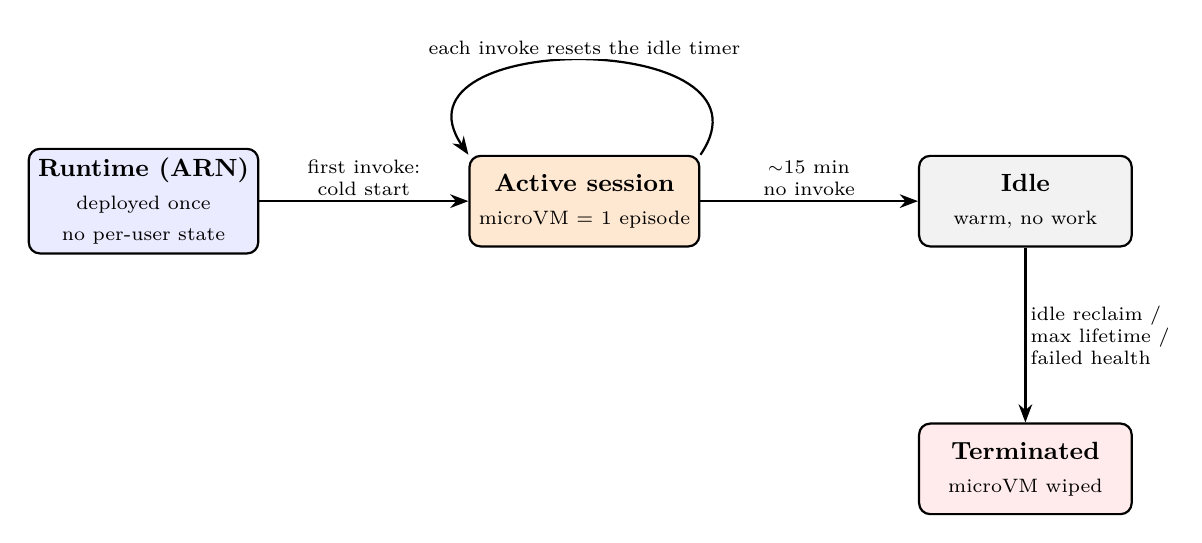
\begin{tikzpicture}[
  font=\small,
  box/.style={draw, rounded corners, minimum height=1.15cm, minimum width=2.7cm, align=center, thick, fill=white},
  rt/.style={box, fill=blue!8},
  act/.style={box, fill=orange!18},
  idle/.style={box, fill=black!5},
  term/.style={box, fill=red!8},
  lbl/.style={font=\scriptsize, align=center, fill=white, inner sep=1.5pt},
  >={Stealth[]},
]
\node[rt]   (rt)   at (0,0)    {\textbf{Runtime (ARN)}\\[1pt]\scriptsize deployed once\\\scriptsize no per-user state};
\node[act]  (act)  at (5.6,0)  {\textbf{Active session}\\[1pt]\scriptsize microVM = 1 episode};
\node[idle] (idle) at (11.2,0) {\textbf{Idle}\\[1pt]\scriptsize warm, no work};
\node[term] (term) at (11.2,-3.4){\textbf{Terminated}\\[1pt]\scriptsize microVM wiped};
\draw[->, thick] (rt)  -- node[lbl,above]{first invoke:\\cold start} (act);
\draw[->, thick] (act) -- node[lbl,above]{$\sim$15 min\\no invoke} (idle);
\draw[->, thick] (idle) -- node[lbl,right,align=left]{idle reclaim /\\max lifetime /\\failed health} (term);
\draw[->, thick] (act.north east) .. controls +(1.1,1.6) and +(-1.1,1.6) ..
      node[lbl,above]{each invoke resets the idle timer} (act.north west);
\end{tikzpicture}%
}
\end{center}

\emph{Launch is \textbf{implicit} (first invoke); terminate is
\textbf{implicit} (idle / max-lifetime / health). A heartbeat ping
resets the timer (\texttt{demo\_cpu\_quiesce}).}
\end{frame}

\begin{frame}[fragile,allowframebreaks]{How to launch \& terminate a session --- the
mechanics}
\protect\hypertarget{how-to-launch-terminate-a-session-the-mechanics}{}
\begin{itemize}
\tightlist
\item
  \textbf{Launch = the first \texttt{invoke\_agent\_runtime} on a fresh
  \texttt{runtimeSessionId}.} There is no explicit ``start'' call; the
  id (≥33 chars) \emph{is} the launch. The first op cold-starts the
  microVM (or GPU instance --- minutes on a cold GPU); every later op
  with that id re-routes to the same warm box.
\item
  \textbf{Terminate = passive.} No explicit stop on the happy path ---
  the session ends on \textbf{idle reclaim (\textasciitilde15 min)},
  \textbf{max lifetime} (8 h microVM / 14 d instance), or \textbf{failed
  health}. Each invoke resets the idle timer.
\item
  \textbf{Consequence in the RL loop:} a \textbf{100-row dataset does
  not launch 100 instances} --- only \texttt{CONC} episodes are in
  flight, recycling through rows over steps. \textbf{Concurrency
  multiplies instances, not data.}
\item
  The \textbf{weight-sync pause can trip the idle clock} and silently
  lose a warm session → the resilience levers in §5.
\item
  \textbf{Latency: measure, don't assume} --- every op is instrumented
  (\texttt{sandbox\_ms}, \texttt{sglang\_gen\_ms}).
\end{itemize}
\end{frame}

\hypertarget{integrating-agentcore-into-slime-as-the-sandbox}{%
\section{4. Integrating AgentCore into slime as the
sandbox}\label{integrating-agentcore-into-slime-as-the-sandbox}}

\begin{frame}[fragile,allowframebreaks]{How AgentCore sessions integrate into slime ---
the call path}
\protect\hypertarget{how-agentcore-sessions-integrate-into-slime-the-call-path}{}
\begin{center}
\resizebox{0.80\textwidth}{!}{%
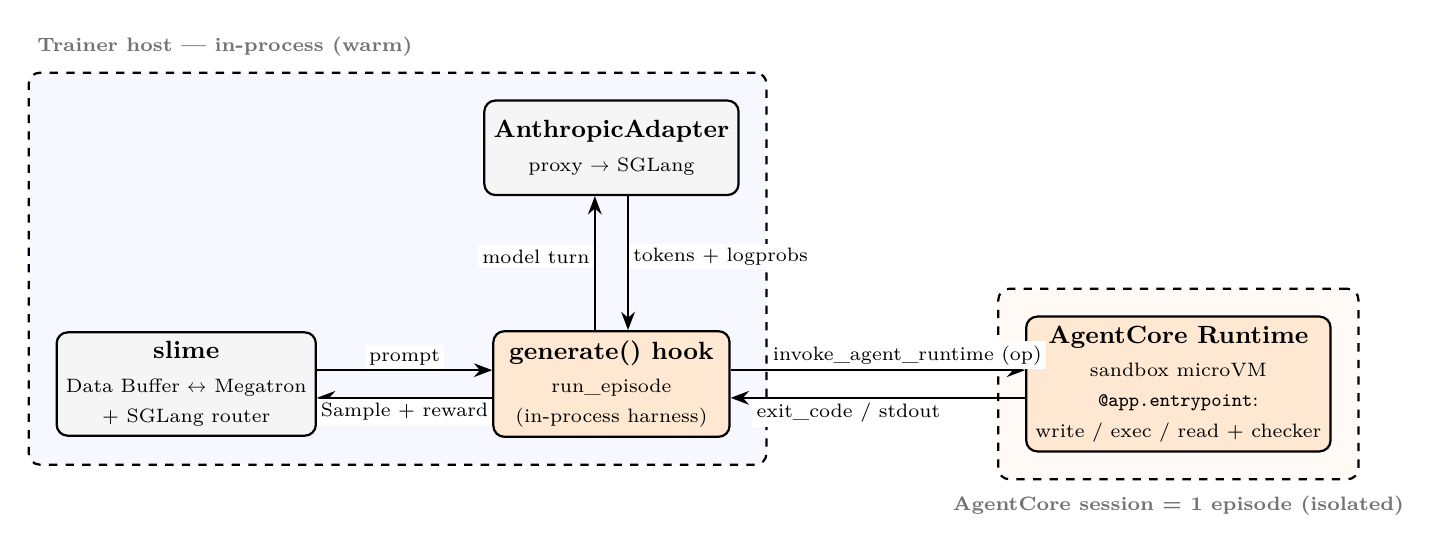
\begin{tikzpicture}[
  font=\small,
  box/.style={draw, rounded corners, minimum height=1.2cm, minimum width=3.0cm, align=center, thick, fill=white},
  gpu/.style={box, fill=blue!8},
  cpu/.style={box, fill=black!4},
  focus/.style={box, fill=orange!18},
  lbl/.style={font=\scriptsize, align=center, fill=white, inner sep=1.5pt},
  ptitle/.style={font=\scriptsize\bfseries, text=black!55},
  panel/.style={draw, rounded corners, dashed, thick, inner sep=0.34cm},
  >={Stealth[]},
]
\node[cpu]   (slime)  at (0,0)     {\textbf{slime}\\[1pt]\scriptsize Data Buffer $\leftrightarrow$ Megatron\\\scriptsize + SGLang router};
\node[focus] (hook)   at (5.4,0)   {\textbf{generate() hook}\\[1pt]\scriptsize run\_episode\\\scriptsize (in-process harness)};
\node[cpu]   (proxy)  at (5.4,3.0) {\textbf{AnthropicAdapter}\\[1pt]\scriptsize proxy $\rightarrow$ SGLang};
\node[focus] (sbx)    at (12.6,0)  {\textbf{AgentCore Runtime}\\[1pt]\scriptsize sandbox microVM\\\scriptsize \texttt{@app.entrypoint}:\\\scriptsize write / exec / read + checker};
\draw[->, thick] ([yshift=5pt]slime.east) -- node[lbl,above]{prompt} ([yshift=5pt]hook.west);
\draw[->, thick] ([yshift=-5pt]hook.west) -- node[lbl,below]{Sample + reward} ([yshift=-5pt]slime.east);
\draw[->, thick] ([xshift=-6pt]hook.north) -- node[lbl,left,pos=0.55]{model turn} ([xshift=-6pt]proxy.south);
\draw[->, thick] ([xshift=6pt]proxy.south) -- node[lbl,right,pos=0.45]{tokens + logprobs} ([xshift=6pt]hook.north);
\draw[->, thick] ([yshift=5pt]hook.east) -- node[lbl,above,pos=0.6]{invoke\_agent\_runtime (op)} ([yshift=5pt]sbx.west);
\draw[->, thick] ([yshift=-5pt]sbx.west) -- node[lbl,below,pos=0.6]{exit\_code / stdout} ([yshift=-5pt]hook.east);
\begin{scope}[on background layer]
  \node[panel, fill=blue!3,   fit=(slime)(proxy)(hook)] (phost) {};
  \node[panel, fill=orange!4, fit=(sbx)]                (psbx)  {};
\end{scope}
\node[ptitle, anchor=south west] at ([yshift=2pt]phost.north west) {Trainer host --- in-process (warm)};
\node[ptitle, anchor=north] at ([yshift=-2pt]psbx.south) {AgentCore session = 1 episode (isolated)};
\end{tikzpicture}%
}
\end{center}

\emph{One \texttt{generate()} hook, one
\textbf{\texttt{runtimeSessionId} per episode}; each tool call = one
SigV4 \texttt{invoke\_agent\_runtime}.}
\end{frame}

\begin{frame}[fragile,allowframebreaks]{Plugging into slime --- one hook, no fork}
\protect\hypertarget{plugging-into-slime-one-hook-no-fork}{}
slime exposes the rollout as a \textbf{custom generation function}, so
the agentic workload plugs in without touching the training kernel:

\begin{itemize}
\tightlist
\item
  \texttt{-\/-custom-generate-function-path\ …generate.generate} ---
  drives the in-process harness; each tool call → one
  \texttt{invoke\_agent\_runtime} keyed by that episode's
  \textbf{\texttt{runtimeSessionId}}.
\item
  \textbf{Design choice:} AgentCore is the \textbf{sandbox, not the
  harness}. The harness stays in-process (warm); the sandbox is the
  isolated per-session microVM. (It \emph{can} host the harness too ---
  \texttt{demo\_cpu\_branching} runs the real Claude Code CLI inside a
  Runtime.)
\item
  The returned \textbf{loss-masked \texttt{Sample} + reward} flows
  straight back into slime's buffer --- no fork of Megatron/SGLang.
\end{itemize}
\end{frame}

\begin{frame}[fragile,allowframebreaks]{Who owns the lifecycle}
\protect\hypertarget{who-owns-the-lifecycle}{}
slime's training kernel controls \textbf{neither} the Runtime nor the
session.

\begin{itemize}
\tightlist
\item
  \textbf{Runtime} (create/delete the ARN) --- the \textbf{deploy
  driver}, once before training. slime just gets the ARN.
\item
  \textbf{Session} (per episode) --- the \texttt{generate} hook's
  sandbox client: \textbf{launch implicit} (first invoke cold-starts the
  microVM); \textbf{terminate implicit} (idle reclaim, no explicit stop
  on the happy path).
\end{itemize}

Because termination is \emph{passive}, the weight-sync pause can trip
the idle clock and lose a warm session --- the failure mode the
resilience demo (\texttt{cpu\_quiesce}) addresses.
\end{frame}

\begin{frame}[allowframebreaks]{The episode, end to end --- the loop}
\protect\hypertarget{the-episode-end-to-end-the-loop}{}
\begin{center}
\resizebox{0.78\textwidth}{!}{%
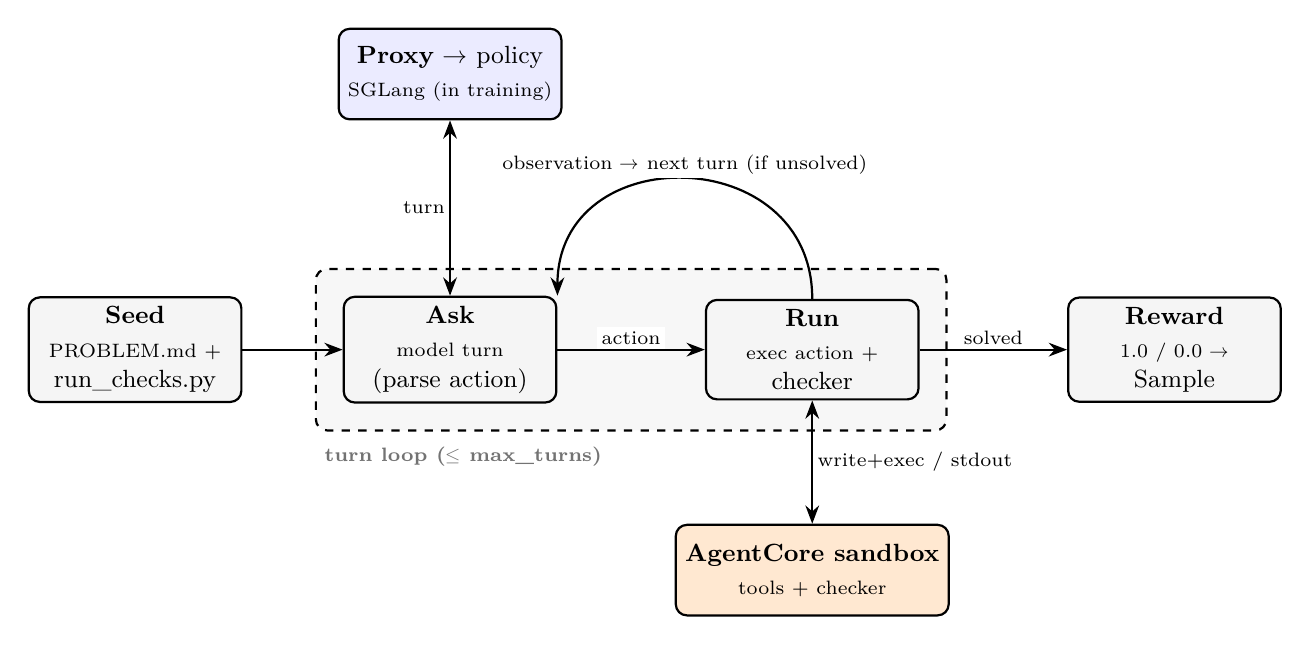
\begin{tikzpicture}[
  font=\small,
  box/.style={draw, rounded corners, minimum height=1.15cm, minimum width=2.7cm, align=center, thick, fill=white},
  svc/.style={box, fill=blue!8},
  focus/.style={box, fill=orange!18},
  stage/.style={box, fill=black!4},
  lbl/.style={font=\scriptsize, align=center, fill=white, inner sep=1.5pt},
  ptitle/.style={font=\scriptsize\bfseries, text=black!55},
  panel/.style={draw, rounded corners, dashed, thick, inner sep=0.34cm},
  >={Stealth[]},
]
\node[stage]  (seed)   at (0,0)     {\textbf{Seed}\\[1pt]\scriptsize PROBLEM.md +\\run\_checks.py};
\node[stage]  (ask)    at (4.0,0)   {\textbf{Ask}\\[1pt]\scriptsize model turn\\(parse action)};
\node[stage]  (run)    at (8.6,0)   {\textbf{Run}\\[1pt]\scriptsize exec action +\\checker};
\node[stage]  (reward) at (13.2,0)  {\textbf{Reward}\\[1pt]\scriptsize 1.0 / 0.0 $\rightarrow$\\Sample};
\node[svc]   (proxy)  at (4.0,3.5) {\textbf{Proxy} $\rightarrow$ policy\\[1pt]\scriptsize SGLang (in training)};
\node[focus] (sbx)    at (8.6,-2.8){\textbf{AgentCore sandbox}\\[1pt]\scriptsize tools + checker};
\draw[->, thick] (seed) -- (ask);
\draw[->, thick] (ask)  -- node[lbl,above]{action} (run);
\draw[->, thick] (run)  -- node[lbl,above]{solved} (reward);
\draw[<->, thick] (ask) -- node[lbl,left]{turn} (proxy);
\draw[<->, thick] (run) -- node[lbl,right]{write+exec / stdout} (sbx);
\draw[->, thick] (run.north) .. controls +(0,2.0) and +(0,2.0) ..
      node[lbl,above,pos=0.5]{observation $\rightarrow$ next turn (if unsolved)} (ask.north east);
\begin{scope}[on background layer]
  \node[panel, fill=black!3, fit=(ask)(run)] (ploop) {};
\end{scope}
\node[ptitle, anchor=north west] at ([yshift=-2pt]ploop.south west) {turn loop ($\leq$ max\_turns)};
\end{tikzpicture}%
}
\end{center}

\emph{Seed → Ask (proxy) → Run (sandbox + checker) → Reward; unsolved
loops back.}
\end{frame}

\begin{frame}[fragile,allowframebreaks]{Step-by-step --- one MBPP episode}
\protect\hypertarget{step-by-step-one-mbpp-episode}{}
\begin{enumerate}
\tightlist
\item
  \textbf{Deploy (once):} build the arm64 sandbox image →
  \texttt{CreateAgentRuntime} → get the ARN (the deploy driver, not
  slime).
\item
  \textbf{Launch run:} \texttt{run.sh} sets \texttt{SANDBOX=agentcore},
  \texttt{FAMILY}, \texttt{CONC}, \texttt{EPISODE\_MAX\_TURNS}, then
  \texttt{ray\ job\ submit\ …\ train\_async.py\ -\/-custom-generate-function-path\ …generate.generate}.
\item
  \textbf{Open session:} slime hands a prompt to \texttt{generate()},
  which rebuilds the \texttt{Task} and calls
  \texttt{make\_sandbox("agentcore")} → \textbf{cold-starts} that
  episode's microVM (\texttt{runtimeSessionId}).
\item
  \textbf{Seed:} \texttt{write\_file} \texttt{PROBLEM.md} + hidden
  \texttt{run\_checks.py} into the session.
\item
  \textbf{Turn loop (≤ \texttt{EPISODE\_MAX\_TURNS}):}
  \texttt{policy.complete} via the \textbf{proxy} (TITO tokens) →
  extract \texttt{solution.py} →
  \texttt{exec("python3\ run\_checks.py")} in the sandbox → on failure,
  feed stdout back.
\item
  \textbf{Reward \& learn:} \texttt{exit\_code\ ==\ 0} → \textbf{reward
  1.0/0.0} from the in-sandbox checker → \texttt{build\_token\_stream} →
  loss-masked \texttt{Sample} → buffer → Megatron step → \textbf{weight
  sync} to SGLang.
\end{enumerate}
\end{frame}

\begin{frame}[fragile,allowframebreaks]{Key code (1/2) --- the in-process generate hook}
\protect\hypertarget{key-code-12-the-in-process-generate-hook}{}
slime calls this once per prompt: build the policy at the SGLang router,
open \textbf{one sandbox per episode}, run the loop, return one
loss-masked \texttt{Sample}.

\begin{Shaded}
\begin{Highlighting}[]
\CommentTok{\# agentcore\_slime\_demo/generate.py   ({-}{-}custom{-}generate{-}function{-}path)}
\ControlFlowTok{async} \KeywordTok{def}\NormalTok{ generate(args, sample, sampling\_params, evaluation}\OperatorTok{=}\VariableTok{False}\NormalTok{):}
\NormalTok{    policy  }\OperatorTok{=}\NormalTok{ SGLangPolicy(router\_url}\OperatorTok{=}\SpecialStringTok{f"http://}\SpecialCharTok{\{}\NormalTok{args}\SpecialCharTok{.}\NormalTok{sglang\_router\_ip}\SpecialCharTok{\}}\SpecialStringTok{:}\SpecialCharTok{\{}\NormalTok{args}\SpecialCharTok{.}\NormalTok{sglang\_router\_port}\SpecialCharTok{\}}\SpecialStringTok{"}\NormalTok{,}
\NormalTok{                           model\_path}\OperatorTok{=}\NormalTok{args.hf\_checkpoint)}
\NormalTok{    task    }\OperatorTok{=}\NormalTok{ \_task\_from\_sample(sample)            }\CommentTok{\# rebuild Task from row metadata}
\NormalTok{    sandbox }\OperatorTok{=}\NormalTok{ make\_sandbox(os.environ.get(}\StringTok{"SANDBOX"}\NormalTok{, }\StringTok{"agentcore"}\NormalTok{))}
    \ControlFlowTok{async} \ControlFlowTok{with}\NormalTok{ sandbox }\ImportTok{as}\NormalTok{ sb:                      }\CommentTok{\# one session == one episode}
\NormalTok{        traj }\OperatorTok{=} \ControlFlowTok{await}\NormalTok{ run\_episode(policy, sb, task, sampling\_params)}
\NormalTok{    tokens, resp\_len, loss\_mask, logprobs }\OperatorTok{=}\NormalTok{ build\_token\_stream(traj, tokenizer)}
    \ControlFlowTok{return}\NormalTok{ Sample(tokens}\OperatorTok{=}\NormalTok{tokens, response\_length}\OperatorTok{=}\NormalTok{resp\_len, reward}\OperatorTok{=}\NormalTok{traj.reward,}
\NormalTok{                  loss\_mask}\OperatorTok{=}\NormalTok{loss\_mask, rollout\_log\_probs}\OperatorTok{=}\NormalTok{logprobs)}
\end{Highlighting}
\end{Shaded}

\begin{itemize}
\tightlist
\item
  Loss mask = \textbf{1 on the policy's own tokens, 0 on prompt /
  observation / tool tokens}.
\item
  \texttt{build\_token\_stream} reuses the \textbf{recorded
  \texttt{token\_ids} per turn} --- no re-tokenization (TITO); returns a
  \emph{bare} \texttt{Sample} (slime's async path chokes on nested
  lists).
\end{itemize}
\end{frame}

\begin{frame}[fragile,allowframebreaks]{Key code (2/2) --- the sandbox client \& the
Runtime server}
\protect\hypertarget{key-code-22-the-sandbox-client-the-runtime-server}{}
Each \texttt{write\_file} / \texttt{exec} / \texttt{read\_file} =
\textbf{one SigV4 \texttt{invoke\_agent\_runtime}} {[}D8{]} keyed by the
episode's session id; boto3 offloaded with \texttt{asyncio.to\_thread}
so \texttt{N} episodes run concurrently (with retries for transient
blips + the GPU cold launch).

\begin{Shaded}
\begin{Highlighting}[]
\CommentTok{\# client — agentcore\_runtime\_sandbox.py}
\KeywordTok{def}\NormalTok{ \_invoke\_sync(}\VariableTok{self}\NormalTok{, payload):}
\NormalTok{    resp }\OperatorTok{=} \VariableTok{self}\NormalTok{.\_client.invoke\_agent\_runtime(agentRuntimeArn}\OperatorTok{=}\VariableTok{self}\NormalTok{.\_arn,}
\NormalTok{        runtimeSessionId}\OperatorTok{=}\VariableTok{self}\NormalTok{.\_session\_id,        }\CommentTok{\# \textgreater{}=33 chars; one per episode}
\NormalTok{        payload}\OperatorTok{=}\NormalTok{json.dumps(payload).encode())}
    \ControlFlowTok{return}\NormalTok{ json.loads(resp[}\StringTok{"response"}\NormalTok{].read().decode())}
\end{Highlighting}
\end{Shaded}

\begin{Shaded}
\begin{Highlighting}[]
\CommentTok{\# server (deployed image) — the checker runs HERE, so the microVM is the reward source}
\NormalTok{app }\OperatorTok{=}\NormalTok{ BedrockAgentCoreApp()}
\AttributeTok{@app.entrypoint}
\KeywordTok{def}\NormalTok{ entrypoint(request):        }\CommentTok{\# dispatch on op: ping / write\_file / read\_file / exec}
    \ControlFlowTok{return}\NormalTok{ handle(request)}
\NormalTok{app.run()                       }\CommentTok{\# serves 0.0.0.0:8080  (/invocations + /ping)}
\end{Highlighting}
\end{Shaded}

\textbf{CPU → GPU is one env var} (\texttt{SANDBOX=}) --- zero change to
the loop.
\end{frame}

\begin{frame}[fragile,allowframebreaks]{One image, many tasks \& dependencies}
\protect\hypertarget{one-image-many-tasks-dependencies}{}
\textbf{One microVM = one image per session.} Task diversity is absorbed
\emph{inside} one generic image, in increasing order of how structural
the difference is:

\begin{enumerate}
\tightlist
\item
  \textbf{Files, not images} --- most CPU families (math \texttt{sympy},
  code \texttt{unittest}, SQL \texttt{sqlite3}, tool-use, light CTF)
  share \textbf{one generic Python image}; prompt, seed files, and
  hidden checker are written into \emph{that episode's session}.
\item
  \textbf{Per-session install} --- heavier deps go into the ephemeral
  workspace: \textbf{\texttt{CMD}-time} (the GPU image installs the
  \textasciitilde2.7 GB torch wheel at boot to stay under the
  \textasciitilde2 GB arm64 cap) or \textbf{seed-time}
  \texttt{git\ clone}/\texttt{pip}.
\item
  \textbf{Per-capability image} --- only a genuine substrate difference
  (chiefly the \textbf{GPU} toolchain: \texttt{nvcc} + a real GPU, or a
  prebuilt dependency set) needs a \textbf{second Runtime ARN}
  (\texttt{demo\_cpu\_imagepool}, the GPU demos).
\end{enumerate}
\end{frame}

\hypertarget{the-demos}{%
\section{5. The demos}\label{the-demos}}

\begin{frame}[fragile,allowframebreaks]{The demo set --- 21 demos, one design}
\protect\hypertarget{the-demo-set-21-demos-one-design}{}
Policy always \textbf{Qwen3-4B}, harness \textbf{in-process} (except
\texttt{cpu\_branching}), AgentCore the \textbf{sandbox}; only the
\emph{substrate} and \emph{task} vary.

\begin{itemize}
\tightlist
\item
  \textbf{6 canonical} --- \texttt{cpu\_single} (MBPP),
  \texttt{cpu\_math}, \texttt{gpu\_single} (KernelBench),
  \texttt{gpu\_shared} (Ray farm), \texttt{cpu\_quiesce} +
  \texttt{gpu\_snapshot} (resilience).
\item
  \textbf{8 per-task CPU fan-out} --- one real HF dataset each: gsm8k,
  math500, deepscaler, humaneval, gretelsql, hotpotqa, xlam, mcp.
\item
  \textbf{2 scale a new dimension} --- \texttt{harness\_scale},
  \texttt{mixtask}.
\item
  \textbf{5 substrate/design variants} (newest) ---
  \texttt{cpu\_branching}, \texttt{cpu\_imagepool},
  \texttt{cpu\_customruntime}, \texttt{gpu\_customruntime},
  \texttt{gpu\_local}.
\end{itemize}

\textbf{Honest status:} only \texttt{cpu\_single} and
\texttt{gpu\_single} carry \textasciitilde10-step curves; the rest are
\texttt{NR=3} smoke or ready-to-run recipes.
\end{frame}

\begin{frame}[fragile,allowframebreaks]{Demos (1/3) --- canonical + resilience}
\protect\hypertarget{demos-13-canonical-resilience}{}
\begin{longtable}[]{@{}
  >{\raggedright\arraybackslash}p{(\columnwidth - 8\tabcolsep) * \real{0.2000}}
  >{\raggedright\arraybackslash}p{(\columnwidth - 8\tabcolsep) * \real{0.2000}}
  >{\raggedright\arraybackslash}p{(\columnwidth - 8\tabcolsep) * \real{0.2000}}
  >{\raggedright\arraybackslash}p{(\columnwidth - 8\tabcolsep) * \real{0.2000}}
  >{\raggedright\arraybackslash}p{(\columnwidth - 8\tabcolsep) * \real{0.2000}}@{}}
\toprule\noalign{}
\begin{minipage}[b]{\linewidth}\raggedright
Demo
\end{minipage} & \begin{minipage}[b]{\linewidth}\raggedright
Substrate
\end{minipage} & \begin{minipage}[b]{\linewidth}\raggedright
Task
\end{minipage} & \begin{minipage}[b]{\linewidth}\raggedright
Real use case
\end{minipage} & \begin{minipage}[b]{\linewidth}\raggedright
Status
\end{minipage} \\
\midrule\noalign{}
\endhead
\texttt{cpu\_single} & CPU µVM & MBPP repair & test-driven coding &
\textbf{trained} (10-step) \\
\texttt{cpu\_math} & CPU µVM & math words & math post-training &
smoke \\
\texttt{gpu\_single} & GPU g6 & KernelBench & CUDA kernel agent &
\textbf{trained} (10-step) \\
\texttt{gpu\_shared} & GPU g6 farm & KernelBench & GPU packing (scarce
GPUs) & smoke green (local GPU) \\
\texttt{cpu\_quiesce} & CPU µVM & heartbeat & keep sandbox warm over
sync & offline \\
\texttt{gpu\_snapshot} & GPU inst. & snapshot & survive instance recycle
& offline + real recycle \\
\bottomrule\noalign{}
\end{longtable}
\end{frame}

\begin{frame}[fragile,allowframebreaks]{Demos (2/3) --- per-task CPU fan-out (real HF
datasets)}
\protect\hypertarget{demos-23-per-task-cpu-fan-out-real-hf-datasets}{}
\begin{longtable}[]{@{}
  >{\raggedright\arraybackslash}p{(\columnwidth - 8\tabcolsep) * \real{0.2000}}
  >{\raggedright\arraybackslash}p{(\columnwidth - 8\tabcolsep) * \real{0.2000}}
  >{\raggedright\arraybackslash}p{(\columnwidth - 8\tabcolsep) * \real{0.2000}}
  >{\raggedright\arraybackslash}p{(\columnwidth - 8\tabcolsep) * \real{0.2000}}
  >{\raggedright\arraybackslash}p{(\columnwidth - 8\tabcolsep) * \real{0.2000}}@{}}
\toprule\noalign{}
\begin{minipage}[b]{\linewidth}\raggedright
Demo
\end{minipage} & \begin{minipage}[b]{\linewidth}\raggedright
Substrate
\end{minipage} & \begin{minipage}[b]{\linewidth}\raggedright
Task
\end{minipage} & \begin{minipage}[b]{\linewidth}\raggedright
Real use case
\end{minipage} & \begin{minipage}[b]{\linewidth}\raggedright
Status
\end{minipage} \\
\midrule\noalign{}
\endhead
\texttt{cpu\_gsm8k} & CPU µVM & GSM8K & grade-school math & smoke,
\texttt{eval} 0.91 \\
\texttt{cpu\_math500} & CPU µVM & MATH-500 & competition math & smoke,
\texttt{eval} 0.83 \\
\texttt{cpu\_deepscaler} & CPU µVM & DeepScaleR & scaled math reasoning
& smoke, \texttt{eval} 0.70 \\
\texttt{cpu\_humaneval} & CPU µVM & HumanEval & function-synthesis
coding & smoke, \texttt{eval} 0.81 \\
\texttt{cpu\_gretelsql} & CPU µVM & Gretel SQL & text-to-SQL analytics &
smoke, \texttt{eval} 0.65 \\
\texttt{cpu\_hotpotqa} & CPU µVM & HotpotQA & multi-hop RAG / search &
smoke, \texttt{eval} 0.21 \\
\texttt{cpu\_xlam} & CPU µVM & xLAM-60k & function-calling agent &
smoke, \texttt{eval} 1.00 \\
\texttt{cpu\_mcp} & CPU µVM & ToolACE (MCP) & MCP tool-schema agent &
smoke, \texttt{eval} 1.00 \\
\bottomrule\noalign{}
\end{longtable}
\end{frame}

\begin{frame}[fragile,allowframebreaks]{Demos (3/3) --- scale + substrate / design
variants}
\protect\hypertarget{demos-33-scale-substrate-design-variants}{}
\begin{longtable}[]{@{}
  >{\raggedright\arraybackslash}p{(\columnwidth - 8\tabcolsep) * \real{0.2000}}
  >{\raggedright\arraybackslash}p{(\columnwidth - 8\tabcolsep) * \real{0.2000}}
  >{\raggedright\arraybackslash}p{(\columnwidth - 8\tabcolsep) * \real{0.2000}}
  >{\raggedright\arraybackslash}p{(\columnwidth - 8\tabcolsep) * \real{0.2000}}
  >{\raggedright\arraybackslash}p{(\columnwidth - 8\tabcolsep) * \real{0.2000}}@{}}
\toprule\noalign{}
\begin{minipage}[b]{\linewidth}\raggedright
Demo
\end{minipage} & \begin{minipage}[b]{\linewidth}\raggedright
Substrate
\end{minipage} & \begin{minipage}[b]{\linewidth}\raggedright
Task
\end{minipage} & \begin{minipage}[b]{\linewidth}\raggedright
Real use case
\end{minipage} & \begin{minipage}[b]{\linewidth}\raggedright
Status
\end{minipage} \\
\midrule\noalign{}
\endhead
\texttt{cpu\_harness\_scale} & CPU µVM & DeepScaleR (fixed) & scale the
rollout driver & offline sweep \\
\texttt{cpu\_mixtask} & CPU µVM & math+SQL+CTF+tool & generalist
multi-family stream & remote smoke green \\
\texttt{cpu\_branching} & CPU CLI Runtime & Claude Code CLI & real-CLI
subagents / branching & recipe (fan-out blocker) \\
\texttt{cpu\_imagepool} & CPU µVM ×3 & datasci (pandas/scipy/sklearn) &
capability-routed image pool & recipe (data staged) \\
\texttt{cpu\_customruntime} & CPU µVM & trivial & managed vs custom
Runtime compare & capability compare \\
\texttt{gpu\_customruntime} & GPU inst. & trivial & GPU only via custom
Runtime & capability compare \\
\texttt{gpu\_local} & local 2×GPU farm & KernelBench &
whole-GPU-per-session farm & recipe only \\
\bottomrule\noalign{}
\end{longtable}
\end{frame}

\hypertarget{special-demos-scaling-sandbox-variants}{%
\section{6. Special demos --- scaling \& sandbox
variants}\label{special-demos-scaling-sandbox-variants}}

\begin{frame}[fragile,allowframebreaks]{Episode shape decides what you scale}
\protect\hypertarget{episode-shape-decides-what-you-scale}{}
The task's shape --- not the domain --- sets the config. \textbf{One
microVM serves many families}: the sandbox is task-agnostic
(\texttt{write\_file} / \texttt{exec} / \texttt{read\_file}); task
specificity is \emph{files seeded per episode}, not a new image.

\begin{longtable}[]{@{}
  >{\raggedright\arraybackslash}p{(\columnwidth - 6\tabcolsep) * \real{0.2500}}
  >{\raggedright\arraybackslash}p{(\columnwidth - 6\tabcolsep) * \real{0.2500}}
  >{\raggedright\arraybackslash}p{(\columnwidth - 6\tabcolsep) * \real{0.2500}}
  >{\raggedright\arraybackslash}p{(\columnwidth - 6\tabcolsep) * \real{0.2500}}@{}}
\toprule\noalign{}
\begin{minipage}[b]{\linewidth}\raggedright
Regime
\end{minipage} & \begin{minipage}[b]{\linewidth}\raggedright
Example
\end{minipage} & \begin{minipage}[b]{\linewidth}\raggedright
Bottleneck
\end{minipage} & \begin{minipage}[b]{\linewidth}\raggedright
Scale
\end{minipage} \\
\midrule\noalign{}
\endhead
single-turn, long trace & math, reasoning & \textbf{generation} &
inference \\
few-turn, heavy checker & KernelBench (CUDA) & \textbf{sandbox} &
sandbox / GPU \\
multi-turn, big observations & SWE, RAG, web & context growth & both +
warm session \\
\bottomrule\noalign{}
\end{longtable}

\begin{itemize}
\tightlist
\item
  \textbf{\texttt{-\/-rollout-max-response-len}} --- per-turn generation
  budget; set from the family's p95 per-turn response (math 1k--32k;
  code 100--800; CUDA kernel 200--1k; tool call 50--300).
\item
  \textbf{\texttt{EPISODE\_MAX\_TURNS}} (default 3) --- the single
  biggest lever on episode cost: single-turn → 1; iterative code/SQL →
  3--5; long-horizon SWE/web → 15--50+.
\end{itemize}
\end{frame}

\begin{frame}[fragile,allowframebreaks]{The scaling demo (1/2) --- the concrete setup \&
the three tiers}
\protect\hypertarget{the-scaling-demo-12-the-concrete-setup-the-three-tiers}{}
On the 8×L40S box the demos \textbf{fix trainer, inference, and harness}
and change only the sandbox ARN + task --- the reference-architecture
disaggregation made concrete:

\begin{longtable}[]{@{}
  >{\raggedright\arraybackslash}p{(\columnwidth - 4\tabcolsep) * \real{0.3333}}
  >{\raggedright\arraybackslash}p{(\columnwidth - 4\tabcolsep) * \real{0.3333}}
  >{\raggedright\arraybackslash}p{(\columnwidth - 4\tabcolsep) * \real{0.3333}}@{}}
\toprule\noalign{}
\begin{minipage}[b]{\linewidth}\raggedright
Component
\end{minipage} & \begin{minipage}[b]{\linewidth}\raggedright
Where
\end{minipage} & \begin{minipage}[b]{\linewidth}\raggedright
Config (shared)
\end{minipage} \\
\midrule\noalign{}
\endhead
\textbf{Trainer} & 4 GPUs & Megatron, GRPO,
\texttt{global\_batch\_size=32}, \texttt{ACTOR\_GPUS=4} \\
\textbf{Inference} & 4 GPUs & SGLang, 2 engines, one \textbf{cache-aware
router}, \texttt{ROLLOUT\_GPUS=4} \\
\textbf{Harness} & in-process (CPU) & \texttt{run\_episode}, fully-async
\texttt{MODE=B}, \texttt{CONC=4}, \texttt{EPISODE\_MAX\_TURNS=3} \\
\textbf{Sandbox} & \textbf{remote AgentCore} & CPU microVM (arm64)
\textbf{or} GPU \texttt{g6} (amd64); one session/episode \\
\bottomrule\noalign{}
\end{longtable}

\begin{center}
\resizebox{0.6\textwidth}{!}{%
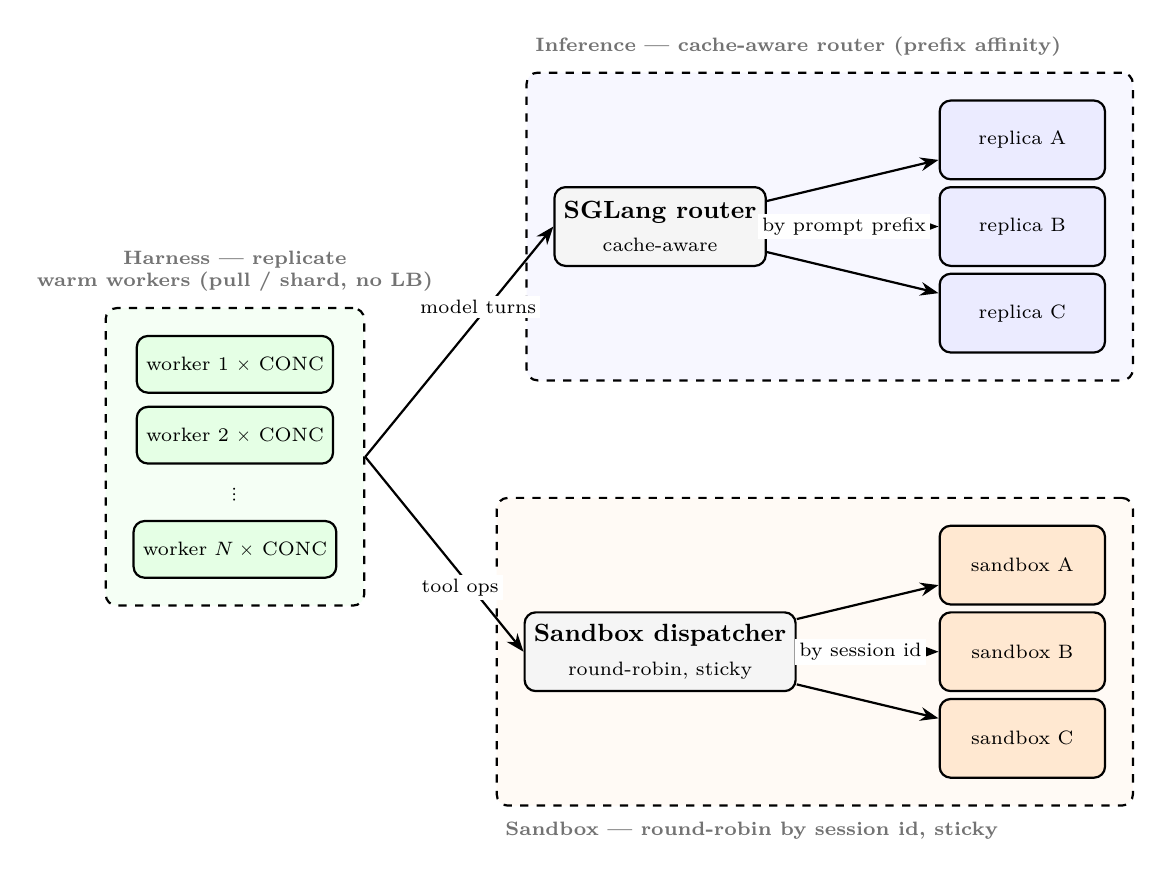
\begin{tikzpicture}[
  font=\small,
  box/.style={draw, rounded corners, minimum height=1.0cm, minimum width=2.5cm, align=center, thick, fill=white},
  gpu/.style={box, fill=blue!8},
  cpu/.style={box, fill=black!4},
  focus/.style={box, fill=orange!18},
  wrk/.style={draw, rounded corners, thick, fill=green!10, minimum height=0.72cm, minimum width=2.3cm, align=center, font=\scriptsize},
  lbl/.style={font=\scriptsize, align=center, fill=white, inner sep=1.5pt},
  ptitle/.style={font=\scriptsize\bfseries, text=black!55, align=center},
  panel/.style={draw, rounded corners, dashed, thick, inner sep=0.34cm},
  >={Stealth[]},
]
\node[wrk] (w1) at (0,0.95) {worker 1 $\times$ CONC};
\node[wrk] (w2) at (0,0.05) {worker 2 $\times$ CONC};
\node[font=\scriptsize] (wd) at (0,-0.7) {$\vdots$};
\node[wrk] (wN) at (0,-1.4) {worker $N$ $\times$ CONC};
\begin{scope}[on background layer]
  \node[panel, fill=green!4, fit=(w1)(w2)(wN)] (harness) {};
\end{scope}
\node[ptitle, anchor=south] at ([yshift=2pt]harness.north) {Harness --- replicate\\warm workers (pull / shard, no LB)};
\node[cpu] (router) at (5.4,2.7) {\textbf{SGLang router}\\[1pt]\scriptsize cache-aware};
\node[gpu, minimum width=2.1cm] (sgA) at (10.0,3.8) {\scriptsize replica A};
\node[gpu, minimum width=2.1cm] (sgB) at (10.0,2.7) {\scriptsize replica B};
\node[gpu, minimum width=2.1cm] (sgC) at (10.0,1.6) {\scriptsize replica C};
\node[cpu] (disp) at (5.4,-2.7) {\textbf{Sandbox dispatcher}\\[1pt]\scriptsize round-robin, sticky};
\node[focus, minimum width=2.1cm] (sbA) at (10.0,-1.6) {\scriptsize sandbox A};
\node[focus, minimum width=2.1cm] (sbB) at (10.0,-2.7) {\scriptsize sandbox B};
\node[focus, minimum width=2.1cm] (sbC) at (10.0,-3.8) {\scriptsize sandbox C};
\draw[->, thick] (harness.east) -- node[lbl,above,pos=0.6]{model turns} (router.west);
\draw[->, thick] (harness.east) -- node[lbl,below,pos=0.6]{tool ops} (disp.west);
\draw[->, thick] (router) -- (sgA);
\draw[->, thick] (router) -- node[lbl,pos=0.45]{by prompt prefix} (sgB);
\draw[->, thick] (router) -- (sgC);
\draw[->, thick] (disp) -- (sbA);
\draw[->, thick] (disp) -- node[lbl,pos=0.45]{by session id} (sbB);
\draw[->, thick] (disp) -- (sbC);
\begin{scope}[on background layer]
  \node[panel, fill=blue!3,   fit=(router)(sgA)(sgC)] (pinf) {};
  \node[panel, fill=orange!4, fit=(disp)(sbA)(sbC)]   (psbx) {};
\end{scope}
\node[ptitle, anchor=south west] at ([yshift=2pt]pinf.north west) {Inference --- cache-aware router (prefix affinity)};
\node[ptitle, anchor=north west] at ([yshift=-2pt]psbx.south west) {Sandbox --- round-robin by session id, sticky};
\end{tikzpicture}%
}
\end{center}

\emph{Each tier balances load by a \textbf{different rule} --- and none
needs a load balancer you build.}
\end{frame}

\begin{frame}[fragile,allowframebreaks]{The scaling demo (2/2) --- the min() law \&
\texttt{cpu\_harness\_scale}}
\protect\hypertarget{the-scaling-demo-22-the-min-law-cpu_harness_scale}{}
\textbf{The min() law ---
\texttt{throughput\ =\ min(inference,\ sandbox,\ harness)}.} Scale two
and the bottleneck moves to the third.

\begin{itemize}
\tightlist
\item
  \textbf{Diagnose first:} compare \texttt{perf/sglang\_gen\_ms\_*} vs
  \texttt{perf/sandbox\_ms\_*}. Generation dominates → add SGLang
  replicas; sandbox dominates → add sessions / ARNs / the GPU farm.
\item
  \textbf{\texttt{cpu\_harness\_scale}} targets the
  \textbf{easily-forgotten third dial}: the warm in-process harness
  (GIL, \texttt{to\_thread} pool, FDs). Scale it by \textbf{replicating
  warm workers} (\texttt{N\ ×\ S}), not by making it ad-hoc.
  \textbf{Problem targeted:} rollout driver becomes the bottleneck once
  inference and sandbox are both fast.
\item
  \textbf{Load-balancing differs by side:} inference → target slime's
  cache-aware router (prefix affinity); sandbox → the \textbf{session id
  \emph{is} the balancer} (sticky round-robin across a pool of ARNs).
  You never stand up your own load balancer.
\end{itemize}
\end{frame}

\begin{frame}[fragile,allowframebreaks]{Special demo --- \texttt{cpu\_mixtask}: the
generalist stream}
\protect\hypertarget{special-demo-cpu_mixtask-the-generalist-stream}{}
\textbf{Real use case:} post-training \textbf{one generalist policy}
across many skills at once --- the frontier norm (Qwen3 {[}3{]},
Nemotron {[}4{]} mix math + code + tool-use + RAG every batch), not one
model per task.

\textbf{Motivation / problem targeted:} a single-task demo can't show
whether the sandbox + reward path stays correct when the batch is
\textbf{heterogeneous} --- different family, checker, and seed files per
row.

\begin{itemize}
\tightlist
\item
  One rollout batch \textbf{spans families} (math + SQL + CTF +
  tool-use) --- no harness or sandbox change; each row carries its own
  family + hidden checker.
\item
  Exercises the claim that \textbf{one generic microVM serves many
  tasks} --- task specificity is \emph{seeded files}, not a new image.
\item
  \textbf{Status:} remote \texttt{NR=3} smoke green.
\end{itemize}
\end{frame}

\begin{frame}[fragile,allowframebreaks]{Special demo --- \texttt{gpu\_shared}: packing
episodes onto one GPU}
\protect\hypertarget{special-demo-gpu_shared-packing-episodes-onto-one-gpu}{}
\textbf{Real use case:} GPU-in-the-loop RL --- a \textbf{CUDA-kernel
agent} (KernelBench {[}7{]}) whose checker \emph{compiles and runs} on a
real GPU, trained when the GPU fleet is scarce or costly.

\textbf{Motivation / problem targeted:} KernelBench is sandbox-bound,
and the isolated path needs \emph{\texttt{N} whole g6 instances at once}
--- which stalls on a \textbf{capacity-starved} fleet (and costs
\texttt{N}×).

\begin{itemize}
\tightlist
\item
  All episodes invoke \textbf{one} GPU Runtime under a \textbf{shared
  \texttt{runtimeSessionId}}; inside, \texttt{\_handle\_farm} leases
  \textbf{one fractional-GPU Ray actor per episode} (keyed by a
  per-episode \texttt{sub\_session}).
\item
  \texttt{num\_gpus=0.5} → two warm-CUDA actors share the GPU;
  \texttt{0.25} → four. \textbf{No MIG on L4}, so isolation is
  software-only (per-process memory caps + an \texttt{nvcc}
  \texttt{flock}).
\item
  \textbf{The trade:} isolated = \texttt{N} clean instances
  (unobtainable when the fleet is starved) vs shared = one instance,
  weaker isolation. \textbf{Primary motivation is capacity, not just
  cost.}
\item
  \textbf{Status:} runs \textbf{end-to-end on hardware} (\texttt{NR=3}
  smoke, \texttt{Job\ succeeded} + ckpt) via the local-GPU fallback;
  fractional packing verified, no convergence curve yet.
  \texttt{gpu\_local} is the same farm on reserved local GPUs at
  fraction=1.0 (one whole GPU per session).
\end{itemize}
\end{frame}

\begin{frame}[fragile,allowframebreaks]{Special demo --- \texttt{cpu\_imagepool}:
capability-routed image pool}
\protect\hypertarget{special-demo-cpu_imagepool-capability-routed-image-pool}{}
\textbf{Real use case:} a \textbf{data-science / analytics agent} whose
tasks each pull a different heavy toolkit (pandas, scipy, sklearn) ---
the reward comes from actually running that stack.

\textbf{Motivation / problem targeted:} those dependency sets are
\textbf{heavy and incompatible} --- they don't all fit under the
\textasciitilde2 GB image cap, and shouldn't co-install in one generic
image.

\begin{itemize}
\tightlist
\item
  \textbf{One prebuilt image per capability}, each its own Runtime ARN
  (datasci→pandas / scipy→scipy / sklearn→sklearn); the harness
  \textbf{routes each episode to the image its family needs}.
\item
  Shows the third rung of the dependency ladder: when
  \emph{files-in-a-session} and \emph{\texttt{CMD}-time install} aren't
  enough, add a \textbf{per-capability ARN} and round-robin the pool.
\item
  \textbf{Status:} deployed as VPC Runtimes (3-image ARN map); recipe
  with data staged.
\end{itemize}
\end{frame}

\begin{frame}[fragile,allowframebreaks]{Special demo --- \texttt{cpu\_branching}: the
real Claude Code CLI as harness}
\protect\hypertarget{special-demo-cpu_branching-the-real-claude-code-cli-as-harness}{}
\textbf{Real use case:} training a \textbf{real production coding agent}
(Claude Code CLI, with subagents + summarization) with RL --- not a toy
in-process loop. This is where AgentCore hosts the \emph{harness}, not
just the sandbox.

\textbf{Motivation / problem targeted:} a real agent \textbf{fans one
episode out into many samples} (spawns subagents, summarizes → resets
the token prefix). Scored naively per-sample, that fan-out silently
reweights the GRPO baseline and the loss {[}1{]}.

\begin{center}
\resizebox{0.66\textwidth}{!}{%
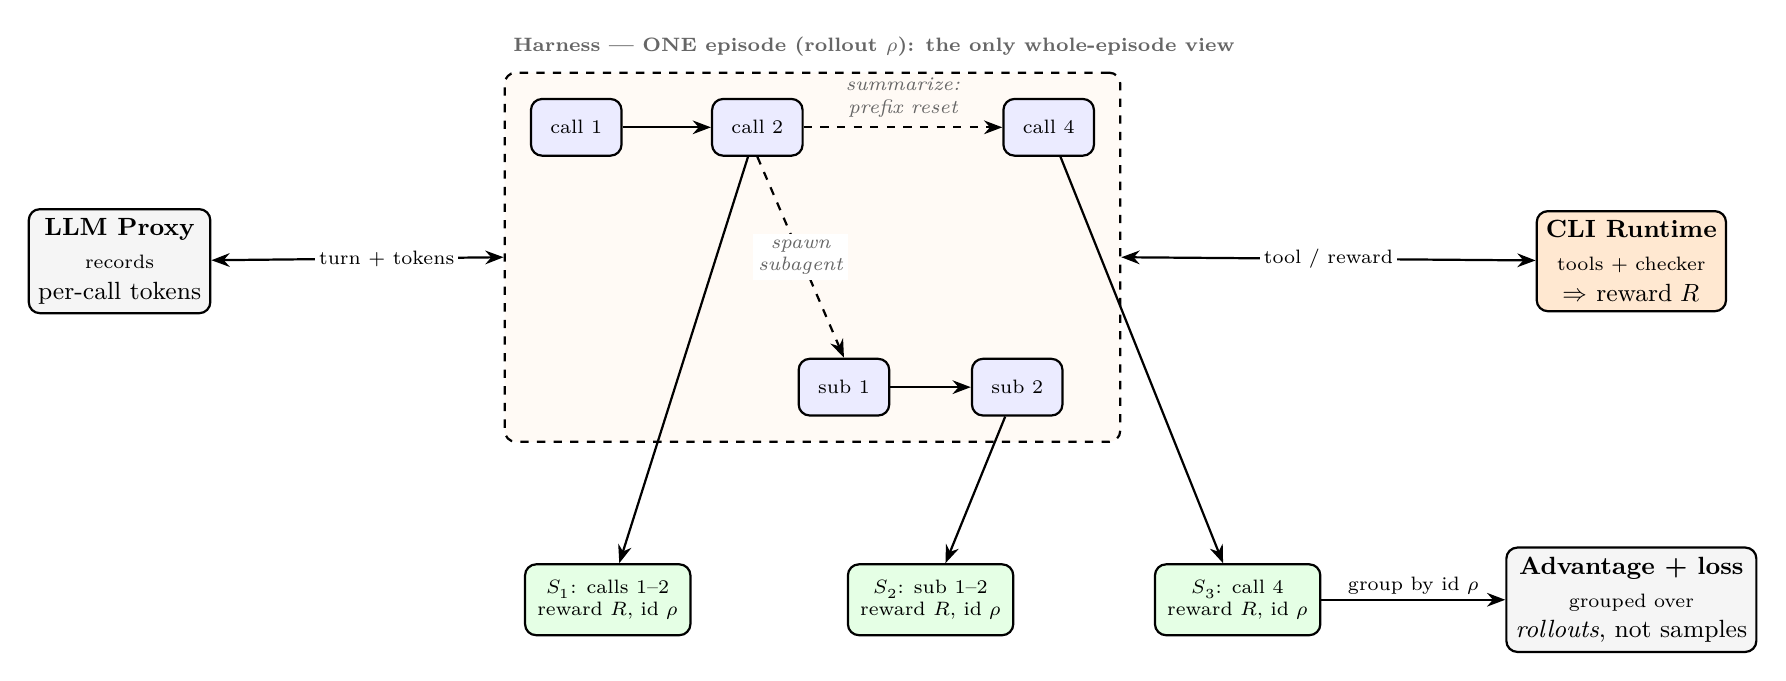
\begin{tikzpicture}[
  font=\small,
  box/.style={draw, rounded corners, minimum height=1.05cm, minimum width=2.2cm, align=center, thick, fill=white},
  cpu/.style={box, fill=black!4},
  focus/.style={box, fill=orange!18},
  call/.style={draw, rounded corners, thick, fill=blue!8, minimum height=0.72cm, minimum width=1.15cm, align=center, font=\scriptsize},
  smp/.style={draw, rounded corners, thick, fill=green!10, minimum height=0.9cm, minimum width=2.1cm, align=center, font=\scriptsize},
  lbl/.style={font=\scriptsize, align=center, fill=white, inner sep=1.5pt},
  op/.style={font=\scriptsize\itshape, text=black!60, align=center},
  panel/.style={draw, rounded corners, dashed, thick, inner sep=0.32cm},
  >={Stealth[]},
]
\node[cpu]   (proxy)   at (-3.6,0.1) {\textbf{LLM Proxy}\\[1pt]\scriptsize records\\per-call tokens};
\node[focus] (sandbox) at (15.6,0.1) {\textbf{CLI Runtime}\\[1pt]\scriptsize tools + checker\\$\Rightarrow$ reward $R$};
\node[call] (c1) at (2.2,1.8) {call 1};
\node[call] (c2) at (4.5,1.8) {call 2};
\node[call] (c3) at (8.2,1.8) {call 4};
\node[call] (s1) at (5.6,-1.5) {sub 1};
\node[call] (s2) at (7.8,-1.5) {sub 2};
\draw[->,thick] (c1)--(c2);
\draw[->,thick,dashed] (c2) -- node[op,above]{summarize:\\prefix reset} (c3);
\draw[->,thick,dashed] (c2.south) -- node[op,fill=white,inner sep=2pt,pos=0.5]{spawn\\subagent} (s1.north);
\draw[->,thick] (s1)--(s2);
\begin{scope}[on background layer]
  \node[panel, fill=orange!4, fit=(c1)(c2)(c3)(s1)(s2)] (harness) {};
\end{scope}
\node[op, anchor=south west, font=\scriptsize\bfseries] at ([yshift=2pt]harness.north west) {Harness --- ONE episode (rollout $\rho$): the only whole-episode view};
\draw[<->,thick] (proxy) -- node[lbl,pos=0.6]{turn + tokens} (harness.west);
\draw[<->,thick] (harness.east) -- node[lbl]{tool / reward} (sandbox);
\node[smp] (S1) at (2.6,-4.2) {$S_1$: calls 1--2\\reward $R$,\ id $\rho$};
\node[smp] (S2) at (6.7,-4.2) {$S_2$: sub 1--2\\reward $R$,\ id $\rho$};
\node[smp] (S3) at (10.6,-4.2) {$S_3$: call 4\\reward $R$,\ id $\rho$};
\node[cpu] (adv) at (15.6,-4.2) {\textbf{Advantage + loss}\\[1pt]\scriptsize grouped over\\\emph{rollouts}, not samples};
\draw[->,thick] (c2) -- (S1);
\draw[->,thick] (s2) -- (S2);
\draw[->,thick] (c3) -- (S3);
\draw[->,thick] (S3) -- node[lbl,above]{group by id $\rho$} (adv);
\end{tikzpicture}%
}
\end{center}

\textbf{Solution:} the CLI runs \textbf{inside a CLI-capable CPU
Runtime} (image bakes node22 + \texttt{claude}); one episode returns a
\texttt{list{[}Sample{]}}, all tagged with the shared
\texttt{rollout\_id\ ρ} and the episode's terminal reward \(R\).
\textbf{Advantage baseline + loss are normalized per rollout, not per
sample} (token-mean loss), so an incidental fan-out can't reweight the
update. \texttt{MODE=A}, \texttt{dp=1} (TP2×PP2), sync save.

\emph{Status: recipe only --- live blocker (in-sandbox CLI exits before
the first model call → \texttt{fan\_out=0}); the empty-group crash is
fixed.}
\end{frame}

\begin{frame}[fragile,allowframebreaks]{Special demo --- \texttt{cpu\_quiesce}: heartbeat
keeps the sandbox warm}
\protect\hypertarget{special-demo-cpu_quiesce-heartbeat-keeps-the-sandbox-warm}{}
\textbf{Real use case:} \textbf{any long RL run} --- a warm, stateful
session (installed deps, seeded repo) must survive the periodic
weight-sync pause instead of cold-starting every round.

\textbf{Motivation / problem targeted:} during \textbf{weight sync}
generation stalls; an idle session is \textbf{reclaimed
(\textasciitilde15 min)} {[}D3{]} and the next round pays a \textbf{cold
start} --- repeatedly.

\begin{itemize}
\tightlist
\item
  A \texttt{SessionKeeper} pings the session on a timer,
  \textbf{resetting the idle clock}, so the \emph{same} warm microVM
  survives the sync pause --- no cold start per round.
\item
  Lives \textbf{outside the harness} (\texttt{KeptSandbox} heartbeat),
  because the stall is a property of the training loop, not the episode.
\item
  Complements \texttt{gpu\_snapshot} (recover a \emph{lost} GPU instance
  via an app-level S3 snapshot): \textbf{heartbeat prevents loss;
  snapshot recovers from it.}
\end{itemize}
\end{frame}

\begin{frame}[fragile,allowframebreaks]{Summary}
\protect\hypertarget{summary}{}
\begin{itemize}
\tightlist
\item
  \textbf{Can:} isolated per-session sandbox for untrusted output (CPU
  default), fully in-account (IAM/SigV4, VPC), long sessions,
  bring-your-own container, \textbf{GPU on Instances}; a one-hook slime
  integration with the harness in-process.
\item
  \textbf{Cannot:} a microVM has no GPU; no cross-session GPU
  fractioning (no MIG on L4); a session can't exceed 8 h without moving
  to Instances (14 d).
\item
  \textbf{How to run:} build a sandbox image → deploy a Runtime (+ GPU
  capacity provider) → seed a task → \texttt{invoke\_agent\_runtime} per
  tool call → in-sandbox checker gives the reward → slime trains via one
  \texttt{generate} hook. \textbf{CPU↔GPU is one env var.}
\end{itemize}

\emph{One image, \texttt{N} sessions, one hook: AgentCore is the
isolated per-episode sandbox; slime does the learning.}
\end{frame}

\hypertarget{references}{%
\section{References}\label{references}}

\begin{frame}[allowframebreaks]{References --- papers, models \& tech reports}
\protect\hypertarget{references-papers-models-tech-reports}{}
\begin{itemize}
\tightlist
\item
  \textbf{{[}1{]} Agent Lightning} --- harnessed agentic RL ·
  \url{https://arxiv.org/abs/2508.03680}
\item
  \textbf{{[}2{]} DeepSeek-R1} · \url{https://arxiv.org/abs/2501.12948}
\item
  \textbf{{[}3{]} Qwen3 Technical Report} ·
  \url{https://arxiv.org/abs/2505.09388}
\item
  \textbf{{[}4{]} Llama-Nemotron} ·
  \url{https://arxiv.org/abs/2505.00949}
\item
  \textbf{{[}5{]} Kimi K2} · \url{https://arxiv.org/abs/2507.20534}
\item
  \textbf{{[}7{]} KernelBench} ·
  \url{https://huggingface.co/datasets/ScalingIntelligence/KernelBench}
\item
  \textbf{{[}8{]} MBPP} · \url{https://arxiv.org/abs/2108.07732}
\item
  \textbf{{[}9{]} slime} --- the trainer ·
  \url{https://github.com/THUDM/slime} · docs
  \url{https://thudm.github.io/slime/}
\item
  \textbf{{[}27{]} SGLang / RadixAttention} ·
  \url{https://arxiv.org/abs/2312.07104} · cache-aware router
  \url{https://lmsys.org/blog/2024-12-04-sglang-v0-4/}
\end{itemize}
\end{frame}

\begin{frame}[allowframebreaks]{References --- RL algorithms \& systems (further reading)}
\protect\hypertarget{references-rl-algorithms-systems-further-reading}{}
\begin{itemize}
\tightlist
\item
  \textbf{{[}13{]} GRPO (DeepSeekMath)} ·
  \url{https://arxiv.org/abs/2402.03300}
\item
  \textbf{{[}14{]} DAPO} · \url{https://arxiv.org/abs/2503.14476}
\item
  \textbf{{[}15{]} GSPO} · \url{https://arxiv.org/abs/2507.18071}
\item
  \textbf{{[}18{]} AReaL} --- asynchronous RL system ·
  \url{https://arxiv.org/abs/2505.24298}
\item
  \textbf{{[}19{]} HybridFlow / veRL} ·
  \url{https://arxiv.org/abs/2409.19256}
\item
  \textbf{{[}22{]} Truncated Importance Sampling} --- train/inference
  mismatch · \url{https://fengyao.notion.site/off-policy-rl}
\item
  \textbf{{[}28{]} APRIL} --- active partial rollouts ·
  \url{https://arxiv.org/abs/2509.18521}
\end{itemize}
\end{frame}

\begin{frame}[fragile,allowframebreaks]{References --- AgentCore docs, SDK \& CLI}
\protect\hypertarget{references-agentcore-docs-sdk-cli}{}
\begin{itemize}
\tightlist
\item
  \textbf{{[}D2{]} Host with Runtime} --- isolation, compute types ·
  \url{https://docs.aws.amazon.com/bedrock-agentcore/latest/devguide/agents-tools-runtime.html}
\item
  \textbf{{[}D3{]} Runtime --- how it works} --- idle 15 m / max 8 h ·
  \url{https://docs.aws.amazon.com/bedrock-agentcore/latest/devguide/runtime-how-it-works.html}
\item
  \textbf{{[}D5{]} Instances (GPU)} ·
  \url{https://docs.aws.amazon.com/bedrock-agentcore/latest/devguide/runtime-instances-how-it-works.html}
\item
  \textbf{{[}D8{]} InvokeAgentRuntime} ·
  \url{https://docs.aws.amazon.com/bedrock-agentcore/latest/APIReference/API_InvokeAgentRuntime.html}
\item
  \textbf{{[}D9{]} CreateAgentRuntime} ·
  \url{https://docs.aws.amazon.com/bedrock-agentcore-control/latest/APIReference/API_CreateAgentRuntime.html}
\item
  \textbf{{[}D13{]} Observability} --- vCPU / GB-hour metrics ·
  \url{https://docs.aws.amazon.com/bedrock-agentcore/latest/devguide/observability.html}
\item
  \textbf{{[}D15{]} Python SDK} --- \texttt{@app.entrypoint} ·
  \url{https://github.com/aws/bedrock-agentcore-sdk-python}
\item
  \textbf{{[}D16{]} AgentCore CLI} --- \texttt{@aws/agentcore} ·
  \url{https://www.npmjs.com/package/@aws/agentcore}
\item
  \textbf{{[}D17{]} Runtime service contract} --- :8080, /invocations,
  /ping ·
  \url{https://docs.aws.amazon.com/bedrock-agentcore/latest/devguide/runtime-service-contract.html}
\end{itemize}
\end{frame}

\end{document}
